% Bản thảo tiếng Việt (để đọc và chốt nội dung trước khi chuyển sang tiếng Anh theo mẫu Springer Nature).
% Biên dịch: python3 docs/paper/build_refs.py docs/paper/vi/manuscript_vi.tex docs/paper/vi/refs_auto.tex
%            cd docs/paper/vi && xelatex manuscript_vi && xelatex manuscript_vi
\documentclass[11pt,a4paper]{article}
\usepackage[a4paper,margin=2.4cm]{geometry}
\usepackage{fontspec}
\usepackage{polyglossia}
\setmainlanguage{vietnamese}
\setmainfont{Liberation Serif}
\setsansfont{Liberation Sans}
\usepackage{amsmath,amsthm}
\usepackage{unicode-math}
\setmathfont{Latin Modern Math}
\usepackage{graphicx,booktabs,multirow,array,threeparttable}
\usepackage[labelfont=bf,labelsep=space,font=small,skip=4pt]{caption}
\usepackage{cite}
\usepackage{xcolor}
\usepackage{url}
\usepackage[hidelinks]{hyperref}
\usepackage{lineno}
\usepackage{setspace}
\setstretch{1.12}
\graphicspath{{../figures/}}
\linenumbers

\theoremstyle{plain}
\newtheorem{proposition}{Mệnh đề}
\newtheorem{corollary}{Hệ quả}
\theoremstyle{definition}
\newtheorem{assumption}{Giả thiết}
\theoremstyle{remark}
\newtheorem{remark}{Nhận xét}
\renewcommand{\proofname}{Chứng minh}

\newcommand{\fmax}{f_{\max}}
\newcommand{\tauh}{\hat{\tau}}
\newcommand{\Reff}{R_{\mathrm{eff}}}
\newcommand{\Fs}{\mathcal{F}}
\newcommand{\todo}[1]{\textcolor{red}{[#1]}}

\begin{document}
\renewcommand{\refname}{Tài liệu tham khảo}

\begin{center}
{\Large\bfseries Khi nào cần suy luận depth? Lập lịch nhận thức theo vùng trống đã quan sát cho quadrotor chi phí thấp dùng depth đơn mắt có độ trễ\par}
\vspace{10pt}
\todo{Tác giả 1}\textsuperscript{1*}, \todo{Tác giả 2}\textsuperscript{1}\\[3pt]
{\small \textsuperscript{1}\todo{Đơn vị, cơ quan, thành phố, quốc gia}\\
\textsuperscript{*}Tác giả liên hệ: \todo{e-mail}; ORCID: \todo{0000-0000-0000-0000}}
\end{center}

\begin{abstract}
\noindent Trên quadrotor chi phí thấp, thông tin vật cản thường được lấy từ một camera và một mạng ước lượng depth đơn mắt; đây là khâu tốn tính toán nhất của vòng điều khiển và có độ trễ khoảng 0.1~s. Chạy mạng ở tần số cố định tiêu tốn tài nguyên cả khi không gian phía trước đã được quan sát. Bài báo đề xuất bộ lập lịch theo vùng phủ: một lần suy luận chỉ được kích hoạt khi đoạn đường đi dự kiến, tính tới quãng cần để dừng sau khi kết quả kế tiếp trả về, không còn nằm trong vùng trống mà các khung gần nhất đã quan sát. Bộ lập lịch có trần tần số cứng và được tích hợp với giới hạn tốc độ theo tầm cảm nhận, bộ nhớ vật cản dạng hình trụ đứng cập nhật Kalman tại thời điểm chụp, bộ điều khiển dự báo theo mô hình 20~Hz và bộ lọc hàm rào cản điều khiển 100~Hz. Chúng tôi chỉ ra rằng điều kiện phủ bảo đảm việc bỏ qua suy luận không làm mất khả năng dừng trong vùng đã quan sát, và kiểm chứng các hệ quả của nó trên 36\,000 lượt bay mô phỏng ghép cặp (ba nhóm kịch bản, mười mức trần tần số, ba tốc độ yêu cầu, bốn cấu hình camera). Ở cùng trần tần số, bộ lập lịch đề xuất dùng 50--72\,\% số lần suy luận của phương án tần số cố định trong kịch bản thường và kịch bản đời thường, với tỉ lệ va chạm không khác biệt có ý nghĩa thống kê; tần số chụp tự tăng theo mật độ vật cản; ở cùng ngân sách tính toán thấp, số lượt thất bại trong kịch bản thường giảm từ 35 xuống 16 trên 720. Camera góc nhìn rộng là điều kiện để mức tiết kiệm suy luận không đi kèm suy giảm an toàn.

\medskip
\noindent\textbf{Từ khoá:} lập lịch nhận thức · ước lượng depth đơn mắt · quadrotor · điều khiển dự báo theo mô hình · hàm rào cản điều khiển · tránh vật cản
\end{abstract}

% =====================================================================================================
\section{Giới thiệu}\label{sec:intro}

Quadrotor chi phí thấp bay ở độ cao thấp giữa cây, nhà và phương tiện cần biết vật cản phía trước, nhưng thường chỉ mang một camera và một bộ xử lý nhúng. Mạng ước lượng depth đơn mắt cho phép dựng thông tin hình học từ một ảnh, song đây là khâu tốn tính toán nhất của vòng nhận thức. Độ trễ nhận thức trên robot dao động từ hàng chục tới hàng trăm mili-giây~\cite{falanga2019}; trên một quadrotor bay nhanh, riêng lượt suy luận của mạng chiếm 38.9~ms trong tổng 41.6~ms từ cảm biến tới kế hoạch~\cite{loquercio2021}. Trên GPU V100, Depth Anything V2 cần từ 60~ms (biến thể Small) đến 213~ms (biến thể Large) mỗi ảnh~\cite{yang2024b}; các mạng chính xác nhất quá chậm cho suy luận thời gian thực trên nền nhúng, và CPU/GPU trên máy còn phục vụ các tác vụ khác~\cite{wofk2019}. Trên một MAV dùng depth đơn mắt với phần tính toán đặt ngoài máy bay (GPU RTX 4090), ước lượng depth mất 0.11--0.16~s mỗi khung cộng 0.12~s trễ camera, và vòng nhận thức đạt 3--4~Hz~\cite{simon2023}.

Độ trễ và tần số nhận thức hữu hạn tác động trực tiếp tới an toàn. Độ trễ tối đa mà robot chịu được liên hệ với tốc độ mong muốn, tầm cảm nhận và giới hạn cơ cấu chấp hành~\cite{falanga2019}, và tốc độ cho phép bị chặn bởi tầm cảm biến, gia tốc phanh và thời gian xử lý~\cite{liu2016}. Trong hệ lái tự động được khảo sát ở~\cite{zhao2021}, tần số camera là tham số nhạy nhất với an toàn trong các tham số phần mềm và phần cứng được xét, và tần số cần thiết phụ thuộc độ khó của kịch bản: trong kịch bản bám xe, 3 khung/s đủ ở mức dễ, trong khi mức khó cần ít nhất 5 khung/s. Đặt tần số cố định theo tình huống khó vì vậy dẫn tới cấp phát thừa ở tình huống dễ; theo ước lượng của Zhuyi, trong các thí nghiệm của họ chỉ 36\,\% tài nguyên nhận thức đã cấp phát là cần thiết tại mọi thời điểm~\cite{hsiao2022}. Với UAV bay giữa các vật cản tĩnh, trong phần lớn thời gian bay không gian phía trước đã được quan sát, và một ảnh mới không làm thay đổi quyết định điều khiển.

Các công trình gắn tần số nhận thức với an toàn đã ước lượng liên tục tần số xử lý khung tối thiểu an toàn~\cite{hsiao2022}, tính hạn chót của chuỗi xử lý từ khoảng cách tới vật cản~\cite{gog2022} hoặc từ tầm nhìn~\cite{boroujerdian2021} cùng với quãng dừng, hoặc chọn chế độ hoạt động của bộ ước lượng cùng với điều khiển dự báo~\cite{pant2021}. Các cách tiếp cận này ước lượng hoặc điều chỉnh tần số hay mức tính toán của một luồng khung tuần hoàn; Zhuyi và D3 suy nhu cầu đó từ các vật đã được phát hiện, và việc xét che khuất và vật chưa được phát hiện được Zhuyi để ngỏ~\cite{hsiao2022}. Trong lập kế hoạch chuyển động, an toàn trong môi trường chưa biết được bảo đảm bằng cách luôn giữ một quỹ đạo dừng hoặc quỹ đạo dự phòng trong vùng đã biết là trống~\cite{liu2016,tordesillas2021}, hoặc bằng cách điều chỉnh quỹ đạo để vùng chưa biết mà nó đi vào được quan sát đủ sớm để dừng~\cite{zhou2021}; các phương pháp này dùng các điều kiện đó để định hình chuyển động, không để quyết định khi nào cần cảm nhận. Phép kiểm tra một điểm có nằm trong vùng trống của các ảnh depth gần đây, không cần hợp nhất thành bản đồ, cũng đã được dùng để truy vấn va chạm khi bay nhanh~\cite{florence2018}, nhưng không để quyết định thời điểm chụp. Câu hỏi của bài báo là: \emph{với một mạng depth có độ trễ và chi phí lớn, khi nào cần chạy một lần suy luận để UAV luôn còn một cách dừng nằm trong không gian đã quan sát?}

Luận điểm của chúng tôi là với vật cản tĩnh, nhu cầu suy luận được xác định bởi hình học chứ không bởi đồng hồ. Một ảnh depth mới chỉ mang thông tin liên quan tới an toàn ở phần không gian mà UAV sắp đi qua và chưa quan sát. Vì kết quả của một lần suy luận chỉ có sau độ trễ $\tau$, phần không gian cần được quan sát là đoạn đường đi dự kiến dài $v\tau + v^2/(2a_b) + d_s$. Khi đoạn này đã nằm trong vùng trống của các khung gần nhất, bỏ qua suy luận không làm mất khả năng dừng; khi nó ra khỏi vùng đó, chỉ một khung mới có thể khôi phục khả năng này. Từ luận điểm trên suy ra ba hệ quả kiểm chứng được: (i) ở cùng trần tần số, lập lịch theo điều kiện này giữ được mức an toàn của nhận thức tần số cố định với ít suy luận hơn; (ii) tần số chụp tự tăng khi vật cản dày lên và giảm ở không gian thoáng; (iii) ở cùng số suy luận, phân bổ khung theo hình học cho tỉ lệ va chạm thấp hơn phân bổ theo thời gian an toàn còn lại tới các vật đã biết.

Đóng góp của bài báo gồm:
\begin{enumerate}
\item Bộ lập lịch suy luận theo vùng phủ cho depth đơn mắt có độ trễ: điều kiện kích hoạt trên vùng trống đã quan sát của các khung gần nhất, có số hạng trễ, trần tần số cứng và chế độ chụp khi gần đứng yên; Mệnh đề~\ref{prop:cov} xác định điều kiện để việc bỏ qua suy luận không làm mất khả năng dừng, và Nhận xét~\ref{rem:cap} làm rõ vai trò của trần tần số và giới hạn tốc độ theo tầm cảm nhận.
\item Một kiến trúc nhận thức--điều khiển đa tần số dùng điều kiện trên: vật cản biểu diễn bằng hình trụ đứng có đầu chưa quan sát, bộ nhớ cập nhật Kalman tại thời điểm chụp, bộ điều khiển dự báo theo mô hình (MPC) 20~Hz với hàng hàm rào cản điều khiển (CBF) rời rạc và ràng buộc dừng cuối, bộ lọc CBF dạng phanh 100~Hz.
\item Một nghiên cứu mô phỏng ghép cặp gồm 36\,000 lượt bay kiểm chứng các hệ quả trên, so sánh với nhận thức tần số cố định và với lập lịch thích nghi theo thời gian an toàn còn lại, và khảo sát bốn cấu hình camera.
\end{enumerate}

Kết quả thu được bằng mô phỏng, với vật cản tĩnh lớn và mô hình sai số tổng hợp của mạng depth; Mệnh đề~\ref{prop:cov} là điều kiện cục bộ cho quyết định lập lịch, không phải chứng nhận an toàn của toàn vòng kín. Mục~\ref{sec:related} tổng quan các công trình liên quan; Mục~\ref{sec:model} mô tả mô hình và bài toán; Mục~\ref{sec:method} trình bày phương pháp; Mục~\ref{sec:setup} mô tả thiết lập thử nghiệm; Mục~\ref{sec:results} kiểm chứng các luận điểm; Mục~\ref{sec:discussion} thảo luận phạm vi và hạn chế.

% =====================================================================================================
\section{Các công trình liên quan}\label{sec:related}

\subsection{Độ trễ, tần số nhận thức và an toàn}

Falanga và cộng sự phân tích tốc độ an toàn tối đa của bài toán cảm nhận--tránh theo độ trễ và tầm cảm nhận, cho thấy tầm quan trọng của độ trễ thấp tăng theo tốc độ và tốc độ an toàn rất nhạy với tầm cảm nhận~\cite{falanga2019}; phân tích giả thiết phát hiện vật cản không bất định~\cite{falanga2019} và dùng mô hình chất điểm, một xấp xỉ bỏ qua động lực học quay của quadrotor~\cite{loquercio2021}. Liu và cộng sự chặn tốc độ bằng điều kiện quãng bay trong thời gian xử lý cộng quãng phanh không vượt tầm cảm biến, và coi không gian chưa biết là bị chiếm để UAV luôn dừng được~\cite{liu2016}. Zhuyi định lượng liên tục tần số xử lý khung tối thiểu an toàn như một kiểm tra trực tuyến~\cite{hsiao2022}; Suraksha cho thấy tần số camera là tham số nhạy nhất với an toàn trong các tham số được khảo sát~\cite{zhao2021}; RoboRun định nghĩa hạn chót quyết định của drone là độ trễ lớn nhất còn bảo đảm bay không va chạm và điều chỉnh tần số quyết định theo sự không đồng nhất của không gian, với tốc độ tối đa chọn bằng thực nghiệm~\cite{boroujerdian2021}. D3 tính hạn chót đầu--cuối từ khoảng cách tới vật cản và quãng dừng, và giảm 68\,\% va chạm so với thực thi tuần hoàn trong mô phỏng vòng kín~\cite{gog2022}. Pant và cộng sự đồng thiết kế điều khiển dự báo bền vững với chế độ hoạt động của bộ ước lượng thị giác, có bảo đảm khả thi đệ quy và thử nghiệm bay thật, trong khi khung hình vẫn được lấy mẫu tuần hoàn~\cite{pant2021}. Aldana-López và cộng sự lập lịch giữa các chế độ nhận thức theo đánh đổi độ trễ--độ chính xác với một tác vụ nhận thức đang xử lý tại mỗi thời điểm, và chỉ ra bài toán lập lịch tối ưu là NP-khó~\cite{aldana2023}. Ở phía điều khiển, bỏ qua tính toán có chứng nhận an toàn đã được đề xuất, trong khi trạng thái vẫn được cảm nhận ở mọi bước~\cite{huang2020}.

Khác với các công trình trên, bộ lập lịch của chúng tôi quyết định tại mỗi bước điều khiển có chạy suy luận hay không, từ một điều kiện hình học trên vùng trống đã quan sát dọc đường đi dự kiến, và được đánh giá vòng kín bằng tỉ lệ va chạm trên quadrotor.

\subsection{Lập kế hoạch trong môi trường chưa biết}

Các bộ lập kế hoạch cục bộ cho quadrotor sinh quỹ đạo trong vùng đã biết của bản đồ~\cite{zhou2019}. Coi không gian chưa biết là bị chiếm bảo đảm UAV luôn dừng được~\cite{liu2016}, nhưng điều kiện dừng trong vùng đã biết là trống có thể giới hạn nghiêm trọng tốc độ~\cite{tordesillas2021}; ngược lại, MonoNav coi vùng chưa thám hiểm là trống~\cite{simon2023}. Trong trường hợp xấu nhất, một vật cản có thể nằm ngay sau biên vùng đã thấy~\cite{liu2016}; FASTER vì thế luôn giữ một quỹ đạo dự phòng dừng trong vùng đã biết là trống, với giả thiết bản đồ không nhiễu và thế giới tĩnh~\cite{tordesillas2021}. RAPTOR xác định điểm mà quỹ đạo dự kiến rời vùng đã biết là trống, nơi trong trường hợp xấu nhất có thể có vật cản chưa biết, kiểm tra UAV còn dừng kịp trước điểm đó khi nó trở nên nhìn thấy được hay không, nếu không thì điều chỉnh quỹ đạo để điểm đó được nhìn thấy sớm hơn; nó cũng lập kế hoạch góc yaw để quan sát các vùng chưa biết liên quan tới chuyến bay~\cite{zhou2021}. NanoMap không hợp nhất các ảnh depth thành bản đồ mà giữ lịch sử các ảnh gần đây cùng các phép biến đổi tư thế tương đối, và kiểm tra một điểm có trống hay không bằng cách chiếu nó vào ảnh (trong trường nhìn ngang và dọc, không bị che, không vượt tầm cảm biến)~\cite{florence2018}. Lin và cộng sự buộc quỹ đạo kế hoạch nằm trong trường nhìn và tầm cảm nhận hiện tại và chạy phát hiện--bám vật cản ở mọi khung 60~Hz~\cite{lin2020}. PAMPC đưa mục tiêu nhận thức vào MPC để định hình chuyển động phục vụ ước lượng thị giác~\cite{falanga2018}. Với trường nhìn hạn chế, chuyển động phải được giới hạn để không va vào vùng mù của cảm biến, và khi trường nhìn hẹp hơn $180^\circ$ thì không còn bảo đảm an toàn hoàn toàn chỉ từ thông tin trong trường nhìn~\cite{misyats2025}. Vùng trống đã quan sát trong bài này dùng cùng phép thử theo từng ảnh như~\cite{florence2018} và cùng lập luận xấu nhất về vùng chưa quan sát như~\cite{liu2016,tordesillas2021,zhou2021}, nhưng với mục đích khác: thay vì truy vấn va chạm hay định hình chuyển động, nó quyết định khi nào cần mở rộng vùng đã quan sát bằng một lần suy luận.

\subsection{Hàm rào cản điều khiển với lấy mẫu, độ trễ và bất định}

CBF cho phép lọc lệnh điều khiển bằng một bài toán quy hoạch toàn phương (QP) với can thiệp tối thiểu~\cite{ames2017,ames2019}. Rào cản dựng từ thao tác phanh tối đa bảo đảm luôn dừng kịp với gia tốc cho phép~\cite{ames2017,wang2017}; dẫn xuất kinh điển giả thiết không có trễ phản ứng~\cite{ames2017}, và xung đột giữa rào cản với giới hạn phanh thường được giải quyết bằng quãng phanh tối thiểu~\cite{xiao2019}. CBF rời rạc trong MPC giúp tránh vật sớm hơn với tầm dự báo ngắn, song ràng buộc chỉ lồi khi CBF tuyến tính và tính khả thi bền vững còn là vấn đề mở~\cite{zeng2021}. Kiến trúc đa tần số kết hợp MPC tần số thấp với CBF tần số cao đạt hiệu năng tương đương MPC phi tuyến tần số cao, và tầng CBF là cần thiết vì siết ràng buộc ở MPC một mình không đủ~\cite{rosolia2020}. Khi thực thi rời rạc, luật điều khiển suy từ điều kiện CBF liên tục có thể mất an toàn, và tập an toàn co lại theo chu kỳ lấy mẫu~\cite{breeden2022}; thiết kế thời gian rời rạc chỉ bảo đảm an toàn tại các thời điểm lấy mẫu; trong ví dụ của~\cite{bahati2024}, bộ điều khiển danh định giữ mẫu vi phạm an toàn ở mọi tần số lấy mẫu được thử, và bảo đảm chỉ có được khi mở rộng tập an toàn hoặc hiệu chỉnh lệnh, và trễ không được xét tới có thể dẫn tới va chạm~\cite{molnar2022}. Điều khiển an toàn kích hoạt theo sự kiện và tự kích hoạt quyết định khi nào cập nhật lệnh điều khiển~\cite{taylor2020,yang2019}; trong bối cảnh an toàn, các sự kiện có thể xảy ra dồn dập và khoảng giữa hai sự kiện có thể tiến về 0~\cite{taylor2020}. Sai số của module nhận thức học được đã được đưa vào CBF dưới dạng tập bị chặn~\cite{dean2021}, và quy tắc chọn thời điểm lấy mẫu dựa trên cận sai số đã được dùng cho điều khiển dựa trên nhận thức~\cite{yang2023}. Biên an toàn suy từ cận sai số ước lượng của bộ lọc Kalman mở rộng~\cite{yaghoubi2021} và nửa không gian phồng theo bất định~\cite{zhu2019} là tiền lệ của ràng buộc vật cản trong bài này. An toàn khi mất quan sát đã được xét bằng nhân an toàn ``nhắm mắt''~\cite{laine2020}. Phép đo tới trễ trong vòng một chu kỳ lấy mẫu được cập nhật chính xác trong khuôn khổ đo không theo thứ tự (OOSM) dưới giả thiết tuyến tính--Gauss và liên kết dữ liệu đúng~\cite{barshalom2002}; với nhiều mục tiêu, lời giải vẫn chính xác trừ khi có hơn một tập đo trễ rơi vào cùng một khoảng~\cite{garcia2021}. Trong bài này, bộ lọc CBF và MPC là các khối đã biết; đóng góp nằm ở việc quyết định khi nào đo.

% =====================================================================================================
\section{Mô hình hệ thống và phát biểu bài toán}\label{sec:model}

\subsection{Quadrotor}

Quadrotor được mô hình là vật rắn 6 bậc tự do khối lượng $m = 1$~kg, với lực cản rotor tuyến tính ($k_d = 0.1$~N\,s/m), lực cản thân bậc hai ($c_q = 0.0306$~N\,s$^2$/m$^2$), trễ bậc nhất của lực đẩy 20~ms và tỉ số lực đẩy/trọng lượng 2.4. Các giới hạn của vòng ngoài được suy ra từ mô hình. Với dự trữ lực đẩy $\eta = 0.4$ dành cho điều khiển tư thế, góc nghiêng tối đa thoả $\cos\theta_{\max} = 1/((1-\eta)\,T/W)$, tức $46^\circ$; gia tốc ngang $a_h = g\tan\theta_{\max} = 10.2$~m/s$^2$, hộp gia tốc theo từng trục $a_{xy} = a_h/\sqrt{2} = 7.2$~m/s$^2$, và gia tốc phanh bảo đảm
\begin{equation}\label{eq:ab}
a_b = 0.9\,(a_{xy} - \delta_a) = 6.2~\text{m/s}^2,
\end{equation}
với $\delta_a = 0.3$~m/s$^2$ là cận sai số bám của vòng trong. Tốc độ tới hạn do lực cản ở góc nghiêng tối đa là 16.7~m/s, và tốc độ tối đa $v_{\max} = 15$~m/s. Ước lượng trạng thái (vị trí, vận tốc, tư thế) là bản sao có nhiễu của trạng thái thật ($\sigma_p = 0.02$~m, $\sigma_v = 0.03$~m/s, $\sigma_{\mathrm{att}} = 0.3^\circ$), đại diện cho một bộ VIO/INS.

\subsection{Camera, mạng depth và độ trễ}\label{sec:camera}

Camera mặc định có góc nhìn $102^\circ\times67^\circ$ (Raspberry Pi Camera Module 3 Wide~\cite{rpi_cm3}), gắn ngóc lên $15^\circ$ để bù góc chúi khi bay; ảnh được thu nhỏ về $320\times180$ trước khi đưa vào mạng, tương ứng góc nhìn dọc $70^\circ$ theo mô hình lỗ kim. Mạng depth được thay bằng một mô hình sai số trên ảnh depth dựng bằng dò tia: (i) disparity được lấy trung bình trên diện tích mỗi pixel, nên vật mảnh hơn một pixel bị pha với nền; (ii) làm mờ tăng theo khoảng cách và làm mờ do chuyển động; (iii) sai số tỉ lệ theo từng khung (độ lệch chuẩn 0.04 trong log depth), độ dịch của nghịch đảo depth theo từng khung (0.002~m$^{-1}$), trường sai số tương quan không gian (0.03), nhiễu pixel ($0.03 + 0.004\,d$) và 2\,\% điểm ngoại lai; (iv) sương mù tuỳ chọn. Thành phần tỉ lệ và độ dịch phản ánh việc các mạng depth tương đối dự đoán disparity chỉ đúng tới một thang đo và một độ dịch chưa biết~\cite{ranftl2020,yang2024a,yang2024b} và chỉ đạt độ chính xác báo cáo sau khi căn chỉnh hai đại lượng này theo từng ảnh~\cite{ranftl2020}. Độ trễ đầu--cuối gồm 10~ms chụp, 10~ms truyền và thời gian suy luận phân bố log-chuẩn với trung bình 80~ms (hệ số biến thiên 0.25, giới hạn 40--300~ms); con số này cùng bậc với 73~ms đo trên máy bay ở~\cite{bhattacharya2024} và 60~ms của biến thể nhỏ nhất của Depth Anything V2 trên GPU V100~\cite{yang2024b}. Mạng nhẹ chuyên dụng có thể nhanh hơn nhiều --- FastDepth đạt 178 khung/s trên GPU Jetson TX2, với cân bằng giữa chi phí tính toán và độ chính xác là thách thức cốt lõi~\cite{wofk2019}; giả thiết 80~ms tương ứng một mạng chính xác hơn hoặc một bộ xử lý dùng chung, và ảnh hưởng của độ trễ lớn hơn được xét qua mạng $640\times360$ (320~ms) ở Mục~\ref{sec:r5}. Tầm phát hiện vật bán kính 1~m (ít nhất 90\,\% số khung) đo trên mô hình là 30~m; vì vật ở xa có thể bị đọc xa hơn tới 15\,\%, tầm tin cậy dùng trong điều khiển là $\Reff = 30/1.15 \approx 26$~m.

\subsection{Phát biểu bài toán}

Các giả thiết của bài toán: (i) vật cản tĩnh và lớn, với bán kính tương đương từ 1~m (cây tán thấp, bụi cây, nhà, xe, container, tảng đá); cột mảnh nằm ngoài phạm vi; (ii) UAV chỉ nhận ảnh depth đầu ra của mạng, không có nhãn vật thể; (iii) tại mỗi thời điểm có nhiều nhất một khung đang được xử lý, như trong mô hình nhận thức của~\cite{aldana2023}; (iv) tần số chụp không vượt trần $\fmax$, đại diện cho ngân sách tính toán của bộ tăng tốc. Nhiệm vụ là bay theo một quỹ đạo đặt từ điểm xuất phát tới đích với tốc độ yêu cầu $v_{\mathrm{des}}$. Mục tiêu là giảm số lần suy luận mỗi nhiệm vụ trong khi giữ tỉ lệ va chạm và tỉ lệ kẹt ở mức của nhận thức tần số cố định cùng trần.

% =====================================================================================================
\section{Phương pháp}\label{sec:method}

\subsection{Kiến trúc đa tần số}

Hình~\ref{fig:arch} mô tả vòng kín. Nhánh nhận thức chạy theo sự kiện: khi bộ lập lịch kích hoạt, camera chụp tại $t_c$, mạng trả ảnh depth tại $t_c+\tau$, ảnh được tự phân đoạn thành các hình trụ đứng và đưa vào bộ nhớ vật cản; mỗi kết quả kèm một lưới depth thô $18\times32$ mô tả vùng trống mà khung đó quan sát. Nhánh điều khiển chạy tuần hoàn: MPC ở 20~Hz, bộ lọc CBF và bộ lập lịch ở 100~Hz, điều khiển tư thế ở 500~Hz. Bộ nhớ cung cấp vật cản cho khối tham chiếu (đường vòng, giới hạn tốc độ), MPC, bộ lọc CBF và bộ lập lịch; MPC cung cấp đường đi dự kiến cho bộ lập lịch. Cấu trúc tầng tối ưu tần số thấp và tầng an toàn tần số cao theo~\cite{rosolia2020}.

\begin{figure}[t]
\centering
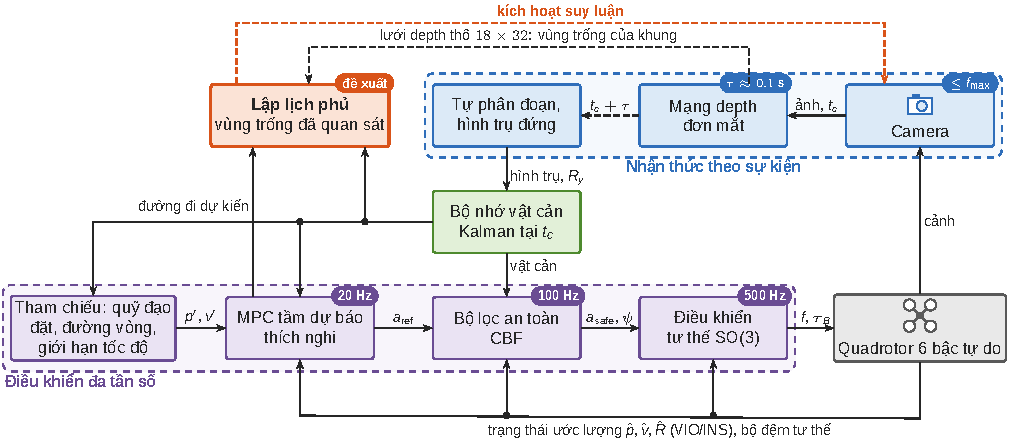
\includegraphics[width=\textwidth]{Fig1_vi.pdf}
\caption{Kiến trúc vòng kín đa tần số. Nhánh nhận thức (khung nét đứt phía trên) chạy theo sự kiện: bộ lập lịch phủ (khối viền đậm, đóng góp của bài) kích hoạt một lần chụp khi đường đi dự kiến rời vùng trống đã quan sát, với tần số không vượt $\fmax$; kết quả của mạng depth tới sau độ trễ $\tau$ và được đưa vào bộ nhớ vật cản bằng cập nhật Kalman tại thời điểm chụp $t_c$. Nhánh điều khiển (khung nét đứt phía dưới) chạy tuần hoàn; nhãn trên mỗi khối là tần số hoặc độ trễ. Mũi tên nét đứt: tín hiệu không đồng bộ}
\label{fig:arch}
\end{figure}

\subsection{Hình trụ đứng và bộ nhớ bù trễ}\label{sec:memory}

\paragraph{Phân đoạn.} Ảnh depth được chia thành các vùng liên thông theo độ lệch log-depth giữa các pixel kề nhau; pixel ngoại lai, pixel ở mép (gradient log-depth lớn) và pixel pha giữa hai bề mặt bị loại; vùng dưới 12 pixel bị bỏ.

\paragraph{Hình trụ.} Phương thẳng đứng lấy từ tư thế tại thời điểm chụp (trên phần cứng: hướng trọng lực của IMU). Với mỗi vùng, gọi $u_p$ là hướng ngang và $r_p$ là tầm ngang của pixel $p$, $\bar u$ là hướng trung bình chuẩn hoá, $\varphi_p = \angle(u_p,\bar u)$ và $\alpha = \max_p\varphi_p + \delta/2$ với $\delta$ là góc một pixel. Một hình trụ đứng bán kính $\rho$ có trục cách camera $D$ theo hướng $\bar u$ được nhìn dưới nửa góc $\alpha$ với $\sin\alpha = \rho/D$, và tia lệch $\varphi_p$ cắt mặt trước tại $r_p = D\,(\cos\varphi_p - \sqrt{\sin^2\alpha - \sin^2\varphi_p})$. Mỗi pixel vì thế cho một ước lượng của $D$, và
\begin{equation}\label{eq:cyl}
\hat D = \operatorname*{median}_{\varphi_p \le 0.8\alpha} \frac{r_p}{\cos\varphi_p - \sqrt{\sin^2\alpha - \sin^2\varphi_p}}, \qquad
\rho = \max\!\Big(\hat D\sin\alpha,\; q_{0.9}\big(\|P_h x_p - \hat D\bar u\|\big) - z_{0.9}\,\sigma_{\mathrm{px}}(\hat D)\,\hat D\Big),
\end{equation}
trong đó $P_h$ là phép chiếu lên mặt phẳng ngang, $q_{0.9}$ là phân vị 90\,\% và số hạng thứ hai phủ 90\,\% số điểm của vùng (trừ độ tản dự kiến của nhiễu pixel) cho các hình dạng khác trụ tròn. Vùng có nửa bề rộng ngang lớn hơn $2~\text{m} + 0.1\times$ khoảng cách được chia đôi theo trục chính, đệ quy, nên một bức tường thành một dãy hình trụ. Đáy và đỉnh là điểm thấp nhất và cao nhất quan sát được. Nếu vùng chạm mép trên hoặc mép dưới của ảnh, hoặc pixel ngay dưới (trên) nó gần camera hơn, đầu tương ứng được coi là chưa quan sát và hình trụ được kéo tới mặt đất (lên cao) cho tới khi đầu đó được quan sát. Nhờ vậy vật thấp như xe và tán cây cao không chặn độ cao bay như khi bao bằng hình cầu. Hiệp phương sai đo $R_y$ gồm các thành phần từ sai số tỉ lệ, độ dịch, trường sai số tương quan, độ lệch ở xa, nhiễu pixel và lượng tử hoá góc.

\paragraph{Bộ nhớ bù trễ.} Mỗi hình trụ là một mốc tĩnh gồm vị trí trục $c$, hiệp phương sai $P$, bán kính $\rho$, đáy và đỉnh. Phép đo $y = \hat p(t_c) + \hat R(t_c)\,(p_{BC} + R_{BC}\,c_C)$ được tạo bằng tư thế ước lượng tại thời điểm chụp lấy từ bộ đệm tư thế; cập nhật Kalman được áp tại $t_c$ lên giá trị dự đoán từ hậu nghiệm gần nhất, rồi dự đoán tới thời điểm hiện tại. Theo định nghĩa ở~\cite{barshalom2002}, một phép đo chỉ là đo không theo thứ tự khi track đã được cập nhật tới thời điểm muộn hơn mốc thời gian của nó; giả thiết một khung đang xử lý loại trừ trường hợp này, nên các phép đo được xử lý theo đúng thứ tự thời gian, và trong ví dụ của~\cite{barshalom2002} cách xử lý theo thứ tự thời gian cho cùng kết quả với bộ xử lý tối ưu. Lời giải chính xác của~\cite{barshalom2002} giả thiết hệ tuyến tính--Gauss, liên kết dữ liệu đúng và độ trễ trong một chu kỳ lấy mẫu. Trong hệ của chúng tôi, liên kết không có định danh, sai số tỉ lệ chung cho mọi vật trong một khung và sai số tư thế tại $t_c$ nằm ngoài các giả thiết đó, nên cập nhật là xấp xỉ. Một phát hiện $k$ chỉ được ghép với track $i$ khi khoảng cách Mahalanobis $e_{ik} = \nu_{ik}^\top S_{ik}^{-1}\nu_{ik} \le 16.27$ ($\chi^2_3$, 99.9\,\%), và phép gán là láng giềng gần nhất tham lam theo chi phí $e_{ik} + \ln\det S_{ik}$. Bán kính được làm mượt với hệ số 0.3; một đầu chưa quan sát được thay bằng giá trị đo ở lần đầu nó được quan sát. Phát hiện không ghép được nhưng nằm trong một hình trụ có sẵn bị bỏ qua; các phát hiện còn lại tạo track mới. Track bị loại khi (a) được dự đoán nằm trong ảnh, không bị che, nhưng không ghép được trong 3 khung liên tiếp, hoặc (b) nằm ngoài trường nhìn và cách UAV hơn 10~m. Giữa hai khung, hiệp phương sai tăng theo nhiễu quá trình.

\paragraph{Hình cầu tương đương cục bộ.} Các khối dùng điều kiện bậc nhất tại vị trí UAV $p$ (bộ lọc CBF, đại lượng rủi ro, bộ lập lịch, giới hạn tốc độ) thay mỗi hình trụ bằng hình cầu cùng bán kính có tâm $c_{\mathrm{eff}} = q - \rho\,n$, với $q$ là điểm gần $p$ nhất trên bề mặt hình trụ và $n$ là pháp tuyến ngoài tại $q$; khi đó $\|p - c_{\mathrm{eff}}\| - \rho$ bằng khoảng cách tới hình trụ và hai gradient trùng nhau. MPC tuyến tính hoá hình trụ tại từng điểm dự đoán theo cùng cách.

\subsection{Lập lịch theo vùng trống đã quan sát}\label{sec:scheduler}

\paragraph{Vùng trống của một khung.} Lưới depth thô $G_k$ của khung $k$ chia ảnh thành $18\times32$ ô; mỗi ô giữ phân vị 20\,\% của các depth hợp lệ trong ô, hoặc $\infty$ nếu dưới 20\,\% số pixel hợp lệ. Lưới được chặn ở $\Reff$ rồi lấy cực tiểu trên lân cận $3\times3$, $\tilde G_k = \min_{3\times3}\min(G_k,\Reff)$, để một ống quanh đường đi, không chỉ đường tâm, phải trống. Gọi $z_k(x)$ là depth của điểm $x$ trong hệ quang học của khung $k$ (theo tư thế tại thời điểm chụp) và $\kappa_k(x)$ là ô mà $x$ chiếu vào. Vùng trống mà khung $k$ quan sát là
\begin{equation}\label{eq:free}
\Fs_k = \big\{x:\ z_k(x) > 0.3~\text{m},\ \kappa_k(x)\ \text{không nằm ở biên lưới},\ z_k(x) + d_s \le \tilde G_k(\kappa_k(x))\big\},
\end{equation}
tức các điểm nằm trước bề mặt đo được ít nhất $d_s$; không gian sau bề mặt (bị che), ngoài trường nhìn hoặc xa hơn $\Reff$ không thuộc $\Fs_k$. Vùng trống đã quan sát tại thời điểm $t$ là hợp của $K = 8$ khung gần nhất đã có kết quả, $\Fs(t) = \bigcup_{k\in\mathcal K(t)}\Fs_k$.

\paragraph{Điều kiện phủ.} Gọi $\sigma_t(s)$ là đường đi dự kiến của MPC tham số hoá theo độ dài cung $s$, với $\sigma_t(0) = p(t)$, được kéo dài thẳng theo hướng cuối nếu ngắn hơn cần thiết, và $v = \|v(t)\|$. Quãng cần quan sát là
\begin{equation}\label{eq:need}
\ell(v) = v\,\tauh + \frac{v^2}{2a_b} + d_s,
\end{equation}
tức quãng bay trong khi chờ kết quả của một khung chụp ngay bây giờ, cộng quãng phanh và lề $d_s = 0.5$~m. Điều kiện phủ là
\begin{equation}\label{eq:cov}
C(t):\qquad \sigma_t(s) \in \Fs(t)\quad \forall s \in [s_0,\ \ell(v)],
\end{equation}
với $s_0 = 1$~m (các điểm gần hơn nằm trong lề an toàn). Ước lượng bảo thủ của độ trễ là $\tauh = \mu_\tau + 2\sigma_\tau$, với $\mu_\tau$, $\sigma_\tau$ cập nhật bằng trung bình trượt hàm mũ (hệ số 0.2) từ độ trễ đo được của mỗi kết quả.

\paragraph{Luật kích hoạt.} Tại mỗi bước điều khiển (100~Hz), một khung được chụp khi
\begin{equation}\label{eq:trig}
\begin{aligned}
\mathrm{trig}(t) &= I(t) \wedge \big[\neg C(t) \vee e_\sigma(t) \vee e_{\mathrm{em}}(t) \vee (v < v_{\mathrm{stall}})\big],\\
I(t) &= (\text{không có khung đang xử lý}) \wedge (t - t_{\mathrm{last}} \ge 1/\fmax).
\end{aligned}
\end{equation}
Sự kiện bất định $e_\sigma$ xảy ra khi một vật có thể quan sát lại, ở gần (khoảng cách bảo thủ dưới 8~m), có độ lệch chuẩn vị trí từ 0.6~m và phương sai lớn hơn hai lần phương sai của một phép đo mới ở khoảng cách đó (lọc theo độ lợi thông tin): vật được thấy lần đầu từ xa giữ hiệp phương sai lớn, và các hình trụ phồng theo bất định có thể đóng các khe hẹp cho tới khi được đo lại từ gần. Sự kiện khẩn cấp $e_{\mathrm{em}}$ xảy ra khi một vật trên hướng va chạm có biên dừng $d^c - d_s - v_c^2/(2a_b) \le 0$, với $d^c$ là khoảng cách bảo thủ và $v_c$ là tốc độ tiếp cận. Khi UAV gần như đứng yên ($v < v_{\mathrm{stall}} = 1$~m/s), khung được chụp liên tục ở $\fmax$ để đo lại các vật xung quanh từ gần. Vật đã biết không tự kích hoạt khung, vì chúng đã nằm trong bộ nhớ. Trần $\fmax$ áp dụng cho mọi sự kiện, kể cả khẩn cấp: trong điều khiển an toàn kích hoạt theo sự kiện, động lực học sai số không nhất thiết triệt tiêu khi đại lượng quyết định việc kích hoạt triệt tiêu, nên các lần cập nhật điều khiển có thể xảy ra dồn dập~\cite{taylor2020}; trần cứng là cận dưới thiết kế của khoảng giữa hai lần chụp.

\paragraph{Tính chất của điều kiện phủ.} Mệnh đề sau nêu điều mà điều kiện~\eqref{eq:cov} bảo đảm.

\begin{assumption}\label{as:cov}
(A1) Vật cản tĩnh. (A2) Mọi điểm của $\Fs(t)$ cách bề mặt vật cản ít nhất $r_b$, bán kính va chạm của UAV. (A3) Trong khoảng $[t, t+\tauh]$, UAV đi dọc $\sigma_t$ với tốc độ không vượt $v = \|v(t)\|$, và có thể giảm tốc dọc $\sigma_t$ với gia tốc $a_b$ từ bất kỳ thời điểm nào. (A4) Đoạn $\sigma_t([0,s_0])$ không va chạm.
\end{assumption}

\begin{proposition}\label{prop:cov}
Giả sử Giả thiết~\ref{as:cov} đúng và $C(t)$ thoả. Với mọi $t_b \in [t, t+\tauh]$, thao tác ``đi theo $\sigma_t$ tới $t_b$ rồi phanh với gia tốc $a_b$'' đưa UAV dừng tại $\sigma_t(s^*)$ với $s^* \le \ell(v) - d_s$, toàn bộ đoạn $\sigma_t([0,s^*])$ không va chạm, và đoạn đường đi phía trước điểm dừng tới $\ell(v)$ nằm trong vùng đã quan sát là trống.
\end{proposition}

\begin{proof}
Theo (A3), quãng bay trong $[t, t_b]$ không vượt $v(t_b - t) \le v\tauh$ và tốc độ tại $t_b$ không vượt $v$, nên quãng phanh không vượt $v^2/(2a_b)$. Do đó $s^* \le v\tauh + v^2/(2a_b) = \ell(v) - d_s$. Với $s\in[s_0, \ell(v)]$, $C(t)$ cho $\sigma_t(s)\in\Fs(t)$; theo (A2) các điểm này cách vật cản ít nhất $r_b$ tại lúc quan sát, và theo (A1) điều này vẫn đúng tại mọi thời điểm sau. Với $s\in[0,s_0]$, kết luận suy ra từ (A4).
\end{proof}

Một khung chụp tại bất kỳ thời điểm nào trong $[t, t+\tauh]$ chỉ trả kết quả sau khoảng $\tau \le \tauh$, nên không thông tin mới nào có thể làm thay đổi khả năng dừng của UAV trước $t + \tauh$. Mệnh đề~\ref{prop:cov} khẳng định rằng khi $C(t)$ thoả, khả năng dừng trong không gian đã quan sát vẫn còn trong suốt khoảng đó mà không cần khung mới; bỏ qua suy luận tại $t$ vì vậy không làm mất gì về khả năng dừng. Khi $C(t)$ không thoả, dữ liệu đã có không đủ để chứng nhận một thao tác dừng như vậy, và chỉ một khung mới có thể mở rộng $\Fs$; luật~\eqref{eq:trig} chụp ngay khi trần cho phép.

\begin{corollary}\label{cor:rate}
Bỏ qua các khung cũ hơn và các sự kiện khác, nếu khung mới nhất quan sát vùng trống dọc đường đi tới độ sâu $D$ tính từ vị trí chụp và UAV bay với tốc độ gần không đổi $v$, thì điều kiện~\eqref{eq:cov} dựa trên khung đó thoả cho tới khi UAV đi được $D - \ell(v)$ kể từ lúc chụp. Khoảng giữa hai lần chụp do sự kiện phủ vì vậy xấp xỉ $(D - \ell(v))/v$, bị chặn dưới bởi $1/\fmax$, và giảm khi $D$ giảm (vật cản dày, che khuất, đường vòng) hoặc khi $v$ tăng.
\end{corollary}

\begin{remark}[Trần tần số và giới hạn tốc độ]\label{rem:cap}
Khi $C(t)$ không thoả nhưng $I(t)$ sai (một khung đang xử lý, hoặc chưa đủ $1/\fmax$ kể từ lần chụp trước), khung cần thiết bị trì hoãn và Mệnh đề~\ref{prop:cov} không còn áp dụng. Giới hạn tốc độ~\eqref{eq:vperc} ở Mục~\ref{sec:speed} bù cho trì hoãn này trong không gian thoáng: nếu vùng trống của khung gần nhất dọc đường đi kéo tới $\Reff$, kết quả kế tiếp tới không muộn hơn $T_r$ sau lần chụp đó, và~\eqref{eq:vperc} bảo đảm UAV vẫn dừng được trong vùng trống của khung đó. Khi vật cản hoặc che khuất làm vùng trống ngắn hơn $\Reff$, trần có thể trì hoãn khung cần thiết, và an toàn dựa vào bộ nhớ và bộ lọc CBF. Dự đoán kiểm chứng được: tỉ lệ va chạm tăng mạnh khi $1/\fmax$ trở nên tương đương thời gian UAV tiêu thụ hết vùng trống ngắn trong vùng dày (Mục~\ref{sec:r1}).
\end{remark}

\begin{remark}[Rời rạc hoá và gia tốc]
Điều kiện~\eqref{eq:cov} được đánh giá ở 100~Hz với tốc độ hiện tại; quãng bay thêm trong một bước, $v\Delta t_c \le 0.15$~m, nhỏ hơn $d_s$, nên điểm dừng vẫn nằm trong đoạn đã kiểm tra. Nếu UAV tăng tốc trong $[t, t+\tauh]$ thì (A3) bị vi phạm; việc đánh giá lại ở mỗi bước làm $\ell(v)$ tăng theo và $C$ sai sớm hơn, nhưng~\eqref{eq:need} không chứa số hạng gia tốc.
\end{remark}

\begin{remark}[Phạm vi]\label{rem:scope}
Mệnh đề~\ref{prop:cov} là về quyết định lập lịch, không phải chứng nhận an toàn của vòng kín: MPC và bộ lọc CBF ràng buộc chuyển động theo các vật trong bộ nhớ, không theo $\Fs$; (A2) có thể bị vi phạm bởi sai số depth; và các quy tắc loại track có thể loại bỏ một vật đã quan sát khỏi bộ nhớ. An toàn vòng kín vì vậy được đánh giá bằng thực nghiệm.
\end{remark}

\begin{figure}[t]
\centering
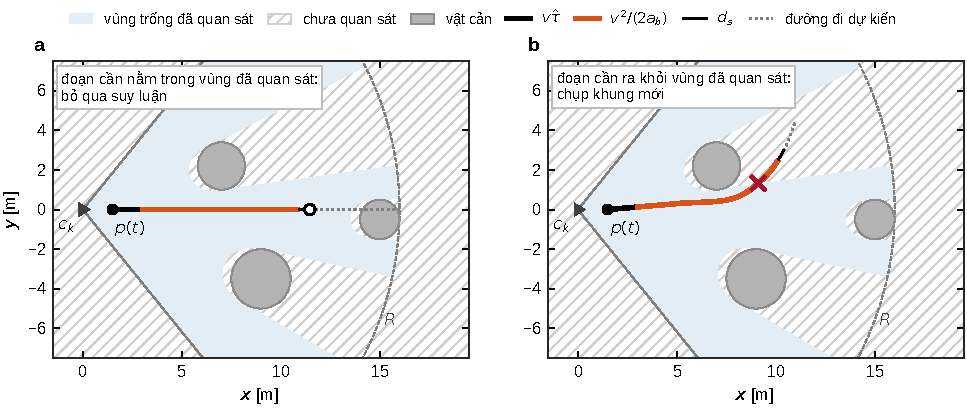
\includegraphics[width=\textwidth]{Fig2.pdf}
\caption{Điều kiện phủ~\eqref{eq:cov}, sơ đồ trên mặt phẳng ngang với một khung chụp tại $c_k$ (góc nhìn $102^\circ$; $R$ tượng trưng cho $\Reff$). Vùng trống đã quan sát kéo tới bề mặt đo được trừ $d_s$; vùng sau vật, ngoài trường nhìn hoặc xa hơn $R$ là chưa quan sát (gạch chéo). UAV ở $p(t)$ với $v = 10$~m/s cần quan sát đoạn đường đi gồm $v\tauh$ (chờ kết quả), $v^2/(2a_b)$ (phanh) và $d_s$. \textbf{a} Đường đi thẳng: cả đoạn cần nằm trong vùng đã quan sát, suy luận được bỏ qua. \textbf{b} Đường vòng ra sau vật: đoạn cần đi vào vùng bị che (dấu $\times$), một khung mới được kích hoạt}
\label{fig:cov}
\end{figure}

\subsection{Giới hạn tốc độ}\label{sec:speed}

Tốc độ tham chiếu là cực tiểu của ba giới hạn. Ngoài giới hạn vật lý $v_{\max}$, giới hạn theo tầm cảm nhận yêu cầu một vật xuất hiện ở biên $\Reff$ vẫn được dừng kịp sau thời gian phản ứng xấu nhất:
\begin{equation}\label{eq:vperc}
v\,T_r + \frac{v^2}{2a_b} + d_s \le \Reff,\qquad T_r = \max(1/\fmax,\ \tauh) + \tauh,
\end{equation}
có cùng dạng với điều kiện của~\cite{liu2016} cộng thêm lề $d_s$; $T_r$ gồm thời gian chờ tới lần chụp kế tiếp (bị chặn bởi trần và bởi khung đang xử lý) cộng độ trễ. Với $\tauh \approx 0.14$~s, giới hạn này là 8.9, 12.1 và 13.5~m/s ở $\fmax = 0.5$, 1 và 1.5~Hz, và vượt $v_{\max}$ từ $\fmax = 3$~Hz. Giới hạn theo mật độ vật cản yêu cầu tốc độ tiếp cận tới mọi vật $i$ trong hành lang bay phía trước đủ để phanh,
\begin{equation}\label{eq:vclut}
v\cos\theta_i \le k_c\sqrt{2a_b\max(d^c_i - d_s,\,0)},\qquad k_c = 0.9,
\end{equation}
với $\theta_i$ là góc giữa hướng bay và hướng tới vật, và không nhỏ hơn 1.5~m/s. Các giới hạn trên dùng mô hình chất điểm và chỉ xét phanh: né ngang tốn ít thời gian hơn phanh ở tốc độ cao~\cite{falanga2019} nên quãng dừng dùng ở đây bảo thủ, còn mô hình chất điểm bỏ qua động lực học quay~\cite{loquercio2021}.

\subsection{Tham chiếu, MPC và bộ lọc CBF}\label{sec:control}

\paragraph{Tham chiếu.} UAV bám quỹ đạo đặt. Khi một đoạn phía trước bị chặn bởi một hình trụ trong bộ nhớ (kể cả lề), tham chiếu chuyển sang đường ngắn nhất không va chạm (đa giác bao các hình trụ ở độ cao bay) tới điểm nhập lại sau đoạn bị chặn, và trong thời gian đó sai lệch so với quỹ đạo đặt không bị phạt. Vật thấp hơn độ cao bay có thể được bay qua.

\paragraph{MPC.} MPC dùng mô hình tích phân kép với bước $\Delta t = 0.1$~s và tầm dự báo $N\in[10,30]$ bước, chọn theo thời gian tới va chạm, quãng phanh và thời điểm kết quả nhận thức kế tiếp được dự kiến tới. Bài toán là
\begin{equation}\label{eq:mpc}
\min_{u,\ s\ge0}\ \sum_{j=1}^{N}\Big(\|p_j - p_j^r\|^2_{Q_p} + \|v_j - v_j^r\|^2_{Q_v} + \|u_{j-1}\|^2_{R} + \|u_{j-1} - u_{j-2}\|^2_{S}\Big) + \sum_i\big(w_1 s_i + w_2 s_i^2\big)
\end{equation}
với ràng buộc hộp trên gia tốc, vận tốc và độ cao, và với mỗi vật $i$ trong 8 vật gần nhất
\begin{subequations}\label{eq:mpccon}
\begin{align}
g_{ij}(p_j) &\ge -s_i, && j = 1,\dots,N, \label{eq:mpca}\\
g_{ij}(p_j) &\ge (1-\gamma)\,g_{ij}(p_{j-1}) - s_i, && j = 1,\dots,N_d, \label{eq:mpcb}\\
\|v_N\|_\infty &\le \varepsilon_v, \label{eq:mpcc}
\end{align}
\end{subequations}
trong đó $g_{ij}(p) = n_{ij}^\top(p - c_{ij}) - d_{ij}$, $c_{ij}$ là tâm hình cầu tương đương của hình trụ tại điểm tuyến tính hoá của bước $j$ (lấy từ nghiệm trước), $n_{ij}$ là pháp tuyến đơn vị của nửa không gian tiếp tuyến (nằm ngang trừ khi vật ở hẳn phía trên hoặc phía dưới, và được xoay sang bên khi gần đối đầu), và $d_{ij} = \rho_i + d_s + \beta\sigma_{ij}$ là bán kính phồng với $\sigma_{ij}$ là độ lệch chuẩn vị trí dự đoán ở bước $j$; $\beta = 2$ là hệ số chọn theo kinh nghiệm, không gắn với một mức xác suất. Ràng buộc~\eqref{eq:mpca} là điều kiện đủ cho $\|p_j - c_{ij}\| \ge d_{ij}$ với mọi pháp tuyến đơn vị và giữ bài toán là QP; \eqref{eq:mpcb} là hàng CBF rời rạc~\cite{zeng2021} trên cùng mặt phẳng ở $N_d = 10$ bước đầu; \eqref{eq:mpcc} yêu cầu kế hoạch kết thúc ở trạng thái dừng, tương ứng với quỹ đạo dừng cam kết của~\cite{liu2016}. Trong $\sigma_{ij}$, hiệp phương sai được giảm tại các bước mà một kết quả nhận thức được dự kiến tới nếu vật nằm trong trường nhìn dự kiến; giá trị trung bình không được cập nhật. Cách phồng theo hiệp phương sai dọc tầm dự báo tương tự~\cite{zhu2019}. Khi bài toán vô nghiệm, một lệnh phanh được dùng thay thế. QP được giải bằng phương pháp điểm trong primal--dual kiểu dự báo--hiệu chỉnh của Mehrotra~\cite{mehrotra1992}, viết bằng MATLAB thuần.

\paragraph{Bộ lọc CBF.} Với mỗi vật trong phạm vi tác dụng, đặt $r = c_{\mathrm{eff}} - p$, khoảng hở $s = \|r\| - d$ với $d = \rho + d_s + \beta\sigma$, và tốc độ tiếp cận $v_c = \hat r^\top v$. Rào cản phanh~\cite{wang2017}
\begin{equation}\label{eq:hbrake}
h = \sqrt{2a_b\,s} - v_c
\end{equation}
dương khi và chỉ khi $v_c^2 < 2a_b s$, tức UAV dừng được trước mặt phồng nếu phanh với gia tốc $a_b$ --- cùng điều kiện phanh với sự kiện khẩn cấp và với giới hạn~\eqref{eq:vclut}. Điều kiện $\dot h \ge -\alpha h$ cho một ràng buộc tuyến tính trên gia tốc lệnh $a$:
\begin{equation}\label{eq:cbfrow}
\hat r^\top a \le \alpha h - \frac{a_b\,(v_c + \dot d)}{\sqrt{2a_b s}} + \frac{\|v_\perp\|^2}{\|r\|} - \delta_a,
\end{equation}
với $v_\perp$ là thành phần vận tốc vuông góc với $\hat r$ và $\dot d$ là tốc độ tăng của bán kính phồng do hiệp phương sai tăng. Bộ lọc giải $\min\|a - a_{\mathrm{ref}}\|^2 + w\,\epsilon^2$ với các hàng~\eqref{eq:cbfrow}, hai hàng giới hạn độ cao và các hàng ``chuyển động mù'' giữ tốc độ đi ngược hướng nhìn của camera dưới 1.5~m/s và tốc độ ra ngoài mép trường nhìn dưới 1~m/s, tương tự ràng buộc giữ vận tốc trong vùng nhìn của cảm biến ở~\cite{misyats2025}. Biến bù $\epsilon$ chỉ khác 0 khi các hàng không tương thích; khi đó lời giải là phương án ít vi phạm nhất~\cite{yaghoubi2021}, không còn bảo đảm $h \ge 0$. Gia tốc an toàn và góc yaw được chuyển thành lực đẩy tổng và tư thế mong muốn của bộ điều khiển bám hình học của~\cite{lee2010}, dùng ở dạng đơn giản hoá (vận tốc góc mong muốn bằng 0 nên các số hạng truyền thẳng triệt tiêu; hệ số theo từng trục; giới hạn nghiêng và lực đẩy; bù lực cản), chạy ở 500~Hz; các kết quả ổn định của~\cite{lee2010} không được viện dẫn cho dạng đơn giản hoá này.

\subsection{Các phương án so sánh}\label{sec:baselines}

\textbf{FR} chụp đều ở đúng $\fmax$. \textbf{RA} (thích nghi theo rủi ro) chọn khoảng quét từ thời gian vòng hở an toàn: với mỗi vật nhìn thấy được, thời gian lớn nhất mà UAV với tốc độ tiếp cận hiện tại vẫn dừng được khi chưa có ảnh mới, có xét hiệp phương sai tăng, cùng với một vật giả định ở biên tầm tin cậy theo hướng bay; khoảng quét là cực tiểu của các thời gian này trừ $\tauh$, kèm các sự kiện khoảng cách, bất định và khẩn cấp. RA tương tự khái niệm cửa sổ an toàn của điều khiển tự kích hoạt~\cite{yang2019} và việc suy tần số tối thiểu từ độ trễ chịu được~\cite{hsiao2022}. \textbf{COV-NC} là COV bỏ giới hạn~\eqref{eq:vclut}. Mọi phương án dùng cùng bộ nhớ, MPC, bộ lọc CBF, giới hạn~\eqref{eq:vperc} và trần $\fmax$. Bảng~\ref{tab:params} liệt kê các tham số chính.

\begin{table}[t]
\centering
\caption{Tham số chính (mọi phương án)}\label{tab:params}
\small
\begin{tabular}{@{}lll@{}}
\toprule
Khối & Tham số & Giá trị \\
\midrule
Quadrotor & khối lượng; $T/W$; bán kính va chạm $r_b$ & 1~kg; 2.4; 0.25~m \\
 & $\theta_{\max}$; $a_b$; $v_{\max}$ & $46^\circ$; 6.2~m/s$^2$; 15~m/s \\
Camera, mạng & góc nhìn; ảnh vào mạng; $\Reff$ & $102^\circ\times70^\circ$; $320\times180$; 26~m \\
 & độ trễ (chụp + truyền + suy luận) & $10 + 10 + 80$~ms (log-chuẩn, CV 0.25) \\
Lập lịch & $\fmax$ (mặc định); $K$; lưới & 0.5--5~Hz (3~Hz); 8 khung; $18\times32$, phân vị 20\,\% \\
 & $d_s$; $s_0$; $v_{\mathrm{stall}}$; $\tauh$ & 0.5~m; 1~m; 1~m/s; $\mu_\tau + 2\sigma_\tau$ \\
Bộ nhớ & cổng $\chi^2_3$; loại sau; quên ngoài trường nhìn & 16.27; 3 khung; 10~m \\
MPC & tần số; $\Delta t$; $N$; $N_d$; $\gamma$; $\beta$ & 20~Hz; 0.1~s; 10--30; 10; 0.3; 2 \\
CBF & tần số; $\alpha$; $\delta_a$ & 100~Hz; 3~s$^{-1}$; 0.3~m/s$^2$ \\
Tư thế & tần số; tích phân mô hình & 500~Hz; RK4, 2~ms \\
\bottomrule
\end{tabular}
\end{table}

% =====================================================================================================
\section{Thiết lập thử nghiệm}\label{sec:setup}

\paragraph{Kịch bản.} Bảng~\ref{tab:grid} tóm tắt ba nhóm kịch bản. SN (bay thường) gồm tuyến 300~m với 1--3 đoạn ở độ cao 2--3.5~m, chia thành các vùng 40--80~m: 35\,\% trống, 40\,\% thưa (1--3 vật), 25\,\% dày (6--12 vật), khe hở từ 3.5~m. SH (khó) có mọi vùng đều dày, sương mù (tầm nhìn 200~m) ở các thế giới có chỉ số lẻ, và hai phương tiện cắt ngang tuyến (2--4~m/s) ở các thế giới có chỉ số chia hết cho 3; phương tiện không được thông báo cho thuật toán và va chạm với chúng được thống kê riêng vì nằm ngoài giả thiết vật tĩnh. SE (đời thường) gồm tuyến thẳng 200~m với sáu loại cảnh, mỗi loại 5 thế giới: bãi trống, một cây trên tuyến, đại lộ hai hàng cây, xe đỗ ven đường và một xe tải trên tuyến, dãy nhà ven tuyến, khe phố.

\paragraph{Lưới thử nghiệm.} Mỗi phương án chạy trên cùng các thế giới, cùng ba tốc độ yêu cầu (6, 10, 15~m/s) và cùng mười mức trần $\fmax$ (0.5--5~Hz, bước 0.5~Hz), nên mọi so sánh là ghép cặp. Phần chính dùng camera mặc định với COV, FR, RA và COV-NC (14\,400 lượt); phần camera chạy COV và FR với ba camera khác (21\,600 lượt); tổng cộng 36\,000 lượt.

\paragraph{Kết cục và độ đo.} Một lượt kết thúc khi tới đích, va chạm (khoảng cách từ thân tới vật bằng 0) hoặc kẹt (tiến dưới 1~m dọc quỹ đạo đặt trong 60~s); thời gian bay không bị giới hạn. Độ đo gồm tỉ lệ va chạm với vật tĩnh, tỉ lệ kẹt, số lần suy luận mỗi nhiệm vụ, tần số chụp thực tế và thời gian tới đích. Các tỉ lệ được so sánh bằng kiểm định Fisher chính xác hai phía trên số lượt. Khi so sánh các phương án, các mức trần 1.5--5~Hz được gộp, vì Mục~\ref{sec:r1} cho thấy đây là vùng mà tỉ lệ va chạm không còn phụ thuộc trần. Không hiệu chỉnh cho kiểm định bội, nên các giá trị $p$ gần 0.05 được diễn giải thận trọng.

\paragraph{Cài đặt.} Toàn bộ thuật toán được viết bằng MATLAB, và mô hình Simulink được sinh từ cùng mã. Lưới thử nghiệm chạy bằng một động cơ mô phỏng MATLAB dùng cùng các hàm và cùng cấu trúc đa tần số với mô hình Simulink, trên GitHub Actions; mô hình quadrotor được tích phân bằng Runge--Kutta bậc 4 với bước 2~ms. Mã nguồn, kết quả từng lượt và các script lập bảng, vẽ hình được công bố cùng bài (mục Khai báo). \todo{Khai báo sử dụng công cụ AI theo yêu cầu của tạp chí --- tác giả hoàn thiện.}

\begin{table}[t]
\centering
\caption{Kịch bản và lưới thử nghiệm}\label{tab:grid}
\small
\begin{threeparttable}
\begin{tabular}{@{}llcl@{}}
\toprule
Kịch bản & Đặc điểm & Thế giới & Lượt (camera mặc định) \\
\midrule
SN & tuyến 300~m; vùng trống / thưa / dày & 60 & 7\,200 \\
SH & mọi vùng dày; sương mù; phương tiện cắt ngang\tnote{a} & 30 & 3\,600 \\
SE & tuyến 200~m; sáu loại cảnh đời thường & 30 & 3\,600 \\
\midrule
\multicolumn{4}{@{}l}{Mỗi thế giới: 3 tốc độ yêu cầu $\times$ 10 mức $\fmax$ $\times$ 4 phương án (COV, FR, RA, COV-NC)} \\
\multicolumn{4}{@{}l}{Phần camera: 3 camera khác $\times$ 2 phương án (COV, FR) trên cùng lưới: 21\,600 lượt} \\
\bottomrule
\end{tabular}
\begin{tablenotes}\footnotesize
\item[a] Va chạm với phương tiện nằm ngoài phạm vi (giả thiết vật tĩnh) và được thống kê riêng.
\end{tablenotes}
\end{threeparttable}
\end{table}

% =====================================================================================================
\section{Kết quả}\label{sec:results}

Mỗi mục dưới đây kiểm chứng một luận điểm: nêu dự đoán suy từ Mục~\ref{sec:method}, phép thử, và kết luận.

\subsection{Cơ chế trên một nhiệm vụ}\label{sec:r0}

Hình~\ref{fig:mission} so sánh COV và FR trên cùng một thế giới SN với $v_{\mathrm{des}} = 10$~m/s và $\fmax = 3$~Hz. FR chụp đều theo $\fmax t$ (108 lần suy luận). COV dồn suy luận vào các đoạn có vật cản và các đoạn vòng tránh, gần như ngừng chụp trên đoạn thoáng từ khoảng 12~s tới 19~s và khi giảm tốc gần đích (64 lần suy luận). Hai phương án giữ khoảng cách tới vật cản nhỏ nhất 1.7~m và 0.7~m, đều lớn hơn $d_s - r_b$, và tới đích sau 33.7~s và 36.4~s. Nhiệm vụ này minh hoạ cơ chế của luận điểm: số khung cần thiết được quyết định bởi lượng không gian chưa quan sát mà đường đi tiêu thụ, không bởi thời gian bay.

\begin{figure}[t]
\centering
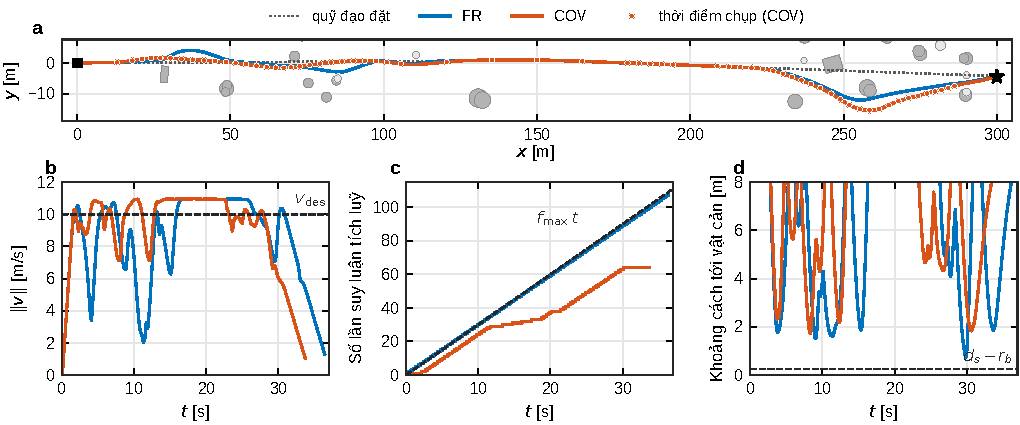
\includegraphics[width=\textwidth]{Fig3.pdf}
\caption{Một nhiệm vụ SN (thế giới 22, $v_{\mathrm{des}} = 10$~m/s, $\fmax = 3$~Hz) với COV và FR. \textbf{a} Quỹ đạo, vật cản (tô đậm: vật cắt độ cao bay) và các thời điểm chụp của COV. \textbf{b} Tốc độ. \textbf{c} Số lần suy luận tích luỹ; nét đứt: $\fmax t$. \textbf{d} Khoảng cách từ thân UAV tới vật cản gần nhất; nét đứt: $d_s - r_b$}
\label{fig:mission}
\end{figure}

\subsection{Luận điểm 1: an toàn cần một tần số tối thiểu và bão hoà trên ngưỡng đó}\label{sec:r1}

\emph{Dự đoán.} Nếu va chạm còn lại do thiếu thông tin mới, tỉ lệ va chạm phải giảm khi tăng trần. Theo Nhận xét~\ref{rem:cap}, điều này chỉ nên đúng ở trần thấp, nơi trần trì hoãn khung cần thiết trong vùng dày.

\emph{Kết quả.} Hình~\ref{fig:rate}a xác nhận dự đoán. Gộp bốn bộ lập lịch, tỉ lệ va chạm trên SN giảm từ 27\,\% ở 0.5~Hz xuống 6.7\,\% ở 1~Hz và 3.8\,\% ở 1.5~Hz (1~Hz so với 1.5~Hz: $p = 0.009$). Từ 2~Hz đến 5~Hz không có khác biệt có ý nghĩa thống kê (SN 3.2\,\% và 2.4\,\%, $p = 0.34$; SH 8.3\,\% và 8.3\,\%, $p = 1$; SE 0.6\,\% và 0.8\,\%, $p = 0.69$). Hình~\ref{fig:rate}b cho thấy COV bị chặn bởi trần ở 0.5~Hz (0.44--0.49 khung/s) và gần trần ở 1~Hz (0.73--0.89 khung/s); từ 1.5~Hz, tần số thực tế tách khỏi trần ngày càng xa và chỉ là 2.3--3.0 khung/s ở 5~Hz. Trần tần số được thoả trong cả 36\,000 lượt: khoảng nhỏ nhất giữa hai lần chụp không nhỏ hơn $1/\fmax$, sai khác không quá một bước điều khiển 10~ms. Ở trần từ 1.5~Hz, tỉ lệ kẹt là 0--0.4\,\% với mọi phương án, trừ COV-NC trên SH (1.2\,\%).

\emph{Kết luận.} Trên khoảng 2~Hz, phần va chạm còn lại không do tần số nhận thức. Khi trần đủ cao để không ràng buộc, COV tự chọn tần số thấp hơn nhiều so với trần.

\begin{figure}[t]
\centering
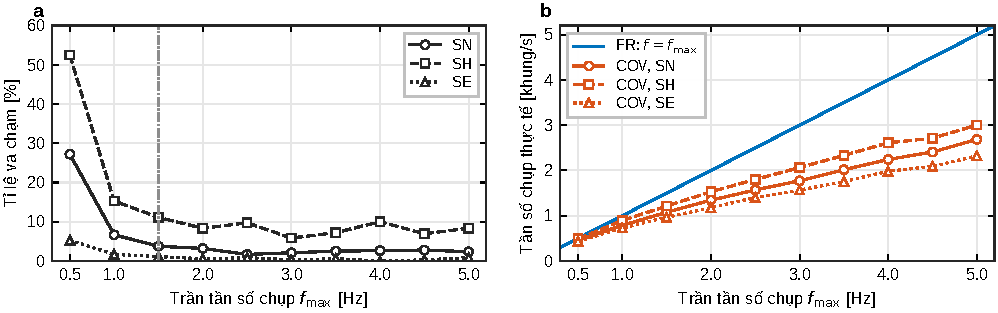
\includegraphics[width=\textwidth]{Fig4.pdf}
\caption{Ảnh hưởng của trần tần số (camera mặc định). \textbf{a} Tỉ lệ va chạm với vật tĩnh, gộp bốn bộ lập lịch (720 lượt mỗi điểm trên SN, 360 trên SH và SE); đường dọc: 1.5~Hz. \textbf{b} Tần số chụp thực tế của COV so với FR, vốn chụp đúng $\fmax$}
\label{fig:rate}
\end{figure}

\subsection{Luận điểm 2: ít suy luận hơn ở cùng mức an toàn}\label{sec:r2}

\emph{Dự đoán.} Theo Mệnh đề~\ref{prop:cov}, ở những thời điểm điều kiện phủ thoả, một khung mới không làm tăng khả năng dừng; FR vẫn chụp ở các thời điểm đó. Với cùng bộ nhớ và cùng các lớp an toàn, COV phải đạt tỉ lệ va chạm tương đương FR cùng trần với ít suy luận hơn.

\emph{Kết quả.} Bảng~\ref{tab:compare} xác nhận dự đoán trên SN và SE. Gộp các trần 1.5--5~Hz, tỉ lệ va chạm tĩnh của COV và FR là 2.4\,\% và 2.0\,\% trên SN ($p = 0.53$), 0.3\,\% và 0.4\,\% trên SE ($p = 1$), trong khi COV dùng 0.54--0.72 (SN) và 0.50--0.63 (SE) số lần suy luận của FR ở cùng trần, tính trên các lượt mà cả hai cùng tới đích. Tỉ lệ này giảm khi trần tăng, vì FR chụp theo trần còn COV chụp theo nhu cầu (Hình~\ref{fig:rate}b). Trên SH, COV dùng 0.61--0.81 số suy luận và có tỉ lệ va chạm 8.2\,\% so với 5.8\,\% ($p = 0.098$): khác biệt không có ý nghĩa ở mức 0.05 nhưng không cho phép kết luận tương đương. Trong cảnh dày liên tục, vùng trống phía trước luôn ngắn, nên phần thời gian mà COV bỏ qua suy luận và mức tiết kiệm đều nhỏ hơn.

So sánh ở cùng trần chưa trả lời câu hỏi thực tế hơn: với một ngân sách tính toán cho trước, nên dùng nó thế nào? Ghép COV ở trần $2f$ với FR ở trần $f$ ($f = 1$, 1.5, 2, 2.5~Hz) cho số suy luận mỗi nhiệm vụ xấp xỉ nhau (trên SN, COV dùng 0.99--1.19 lần số của FR). Trên SN, tổng số lượt thất bại (va chạm tĩnh và kẹt) là 16 so với 35 trên 720 ($p = 0.0096$); chênh lệch tập trung ở cặp 2~Hz--1~Hz, nơi FR nằm trong vùng tần số chưa bão hoà. Trên SH (31 và 43 trên 360, $p = 0.18$, với COV dùng nhiều hơn 7--24\,\% suy luận) và SE (0 và 5 trên 360, $p = 0.062$), khác biệt không có ý nghĩa thống kê.

Giới hạn tốc độ theo mật độ~\eqref{eq:vclut} không tạo khác biệt an toàn có ý nghĩa: COV-NC có tỉ lệ va chạm 2.2\,\%, 7.5\,\% và 0.4\,\% so với 2.4\,\%, 8.2\,\% và 0.3\,\% của COV ($p \ge 0.7$), tỉ lệ kẹt trên SH 1.2\,\% so với 0.3\,\% ($p = 0.064$), và thời gian tới đích ngắn hơn (SN, 15~m/s: 33.5~s so với 36.4~s). Trong lưới này, bộ lọc CBF với cùng điều kiện phanh và giới hạn~\eqref{eq:vperc} đủ để giữ mức an toàn; khối~\eqref{eq:vclut} chủ yếu làm chậm tham chiếu trước khi bộ lọc phải can thiệp.

\emph{Kết luận.} Ở cùng trần, điều kiện phủ loại bỏ 28--50\,\% số lần suy luận trên SN và SE mà không có khác biệt an toàn có ý nghĩa thống kê; với cùng ngân sách, đặt trần cao và để điều kiện phủ quyết định thời điểm chụp không kém, và ở ngân sách thấp tốt hơn, so với chụp đều ở tần số mà ngân sách cho phép.

\begin{table}[t]
\centering
\caption{So sánh các bộ lập lịch ở camera mặc định, gộp $\fmax = 1.5$--5~Hz (SN 1\,440 lượt mỗi phương án; SH và SE 720)}\label{tab:compare}
\small
\begin{threeparttable}
\begin{tabular}{@{}llcccc@{}}
\toprule
Kịch bản & Bộ lập lịch & Va chạm tĩnh [\%] & $p$ so với COV\tnote{a} & Kẹt [\%] & Khung/s\tnote{b} \\
\midrule
\multirow{4}{*}{SN} & COV (đề xuất) & 2.4 & --- & 0.2 & 1.89 \\
 & FR & 2.0 & 0.53 & 0.3 & 3.23 \\
 & RA & 3.9 & 0.033 & 0.3 & 1.89 \\
 & COV-NC & 2.2 & 0.71 & 0.1 & 1.87 \\
\midrule
\multirow{4}{*}{SH} & COV (đề xuất) & 8.2 & --- & 0.3 & 2.16 \\
 & FR & 5.8 & 0.098 & 0.4 & 3.22 \\
 & RA & 12.2 & 0.015 & 0.4 & 2.28 \\
 & COV-NC & 7.5 & 0.70 & 1.2 & 2.16 \\
\midrule
\multirow{4}{*}{SE} & COV (đề xuất) & 0.3 & --- & 0.0 & 1.66 \\
 & FR & 0.4 & 1 & 0.0 & 3.23 \\
 & RA & 1.1 & 0.11 & 0.1 & 1.87 \\
 & COV-NC & 0.4 & 1 & 0.0 & 1.64 \\
\bottomrule
\end{tabular}
\begin{tablenotes}\footnotesize
\item[a] Kiểm định Fisher chính xác hai phía trên số lượt va chạm tĩnh.
\item[b] Tần số chụp trung bình; FR chụp đúng $\fmax$, nên giá trị của FR xấp xỉ trung bình các mức trần (3.25~Hz).
\end{tablenotes}
\end{threeparttable}
\end{table}

\subsection{Luận điểm 3: tần số chụp thích nghi theo mật độ vật cản}\label{sec:r3}

\emph{Dự đoán.} Theo Hệ quả~\ref{cor:rate}, khoảng giữa hai lần chụp của COV giảm khi độ sâu vùng trống phía trước giảm, tức khi vật cản dày lên.

\emph{Kết quả.} Hình~\ref{fig:dens} chia thời gian bay trên SN ($v_{\mathrm{des}} = 15$~m/s, $\fmax = 3$~Hz) theo số vật trong bán kính 15~m. Tần số chụp của COV tăng từ 1.76 khung/s khi không có vật lên 2.59 khung/s khi có từ 6 vật, trong khi FR giữ 2.94--2.99 khung/s bất kể mật độ. Đồng thời, tốc độ trung bình của COV giảm từ 11.2 xuống 3.8~m/s do các giới hạn~\eqref{eq:vperc}--\eqref{eq:vclut} và đường vòng. Theo Hệ quả~\ref{cor:rate}, tốc độ thấp hơn tự nó làm khoảng giữa hai lần chụp dài ra; tần số chụp vẫn tăng, nên mức tăng đến từ vùng trống ngắn hơn và từ các sự kiện bất định, khẩn cấp vốn chỉ xảy ra gần vật cản, chứ không từ tốc độ.

\emph{Kết luận.} Cùng một luật kích hoạt cho tần số thấp ở không gian thoáng và tiến gần trần ở vùng dày --- điều mà tần số cố định chỉ đạt được nếu được đặt theo vùng dày.

\begin{figure}[t]
\centering
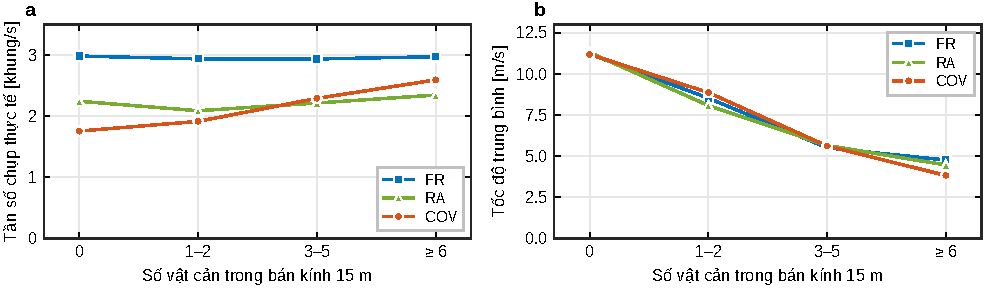
\includegraphics[width=\textwidth]{Fig5.pdf}
\caption{Tần số chụp (\textbf{a}) và tốc độ trung bình (\textbf{b}) theo số vật cản trong bán kính 15~m (SN, $v_{\mathrm{des}} = 15$~m/s, $\fmax = 3$~Hz; toàn bộ thời gian bay trên 60 thế giới)}
\label{fig:dens}
\end{figure}

\subsection{Luận điểm 4: tiêu chí hình học tốt hơn thời gian an toàn còn lại}\label{sec:r4}

\emph{Dự đoán.} RA và COV dùng gần như cùng số suy luận ở cùng trần (tỉ lệ 0.93--0.98 ở 3~Hz), nên so sánh chúng tách được vai trò của \emph{thời điểm} chụp khỏi vai trò của \emph{số} khung. Thời gian an toàn còn lại của RA được tính tới các vật đã có trong bộ nhớ và tới một vật giả định ở biên tầm tin cậy theo hướng bay; nó không xét đường đi thực tế và phần không gian bị che dọc đường đó. Nếu luận điểm đúng, ở cùng số khung, COV phải có tỉ lệ va chạm thấp hơn, đặc biệt khi đường đi rời hướng bay hiện tại.

\emph{Kết quả.} Gộp 1.5--5~Hz, tỉ lệ va chạm của COV thấp hơn RA trên SN (2.4\,\% và 3.9\,\%, $p = 0.033$) và SH (8.2\,\% và 12.2\,\%, $p = 0.015$); trên SE, 0.3\,\% và 1.1\,\% ($p = 0.11$). Hình~\ref{fig:dens}a cho thấy hai bộ lập lịch phân bổ khung khác nhau: RA chụp nhiều hơn COV khi không có vật gần (2.24 và 1.76 khung/s) và ít hơn khi vật dày (2.35 và 2.59 khung/s). Khác biệt này phù hợp với cơ chế của điều kiện~\eqref{eq:cov}: khi đường đi rẽ khỏi hướng bay hiện tại để vòng qua vật, nó đi vào vùng chưa quan sát sau vật (Hình~\ref{fig:cov}b) và điều kiện phủ kích hoạt một khung, trong khi thời gian an toàn còn lại tới các vật đã biết không phụ thuộc vào đường đi. Tình huống này cũng là tình huống quyết định trong thử nghiệm bay của RAPTOR: một vật đặt sau góc khuất chỉ được tránh bởi bộ lập kế hoạch buộc vùng chưa biết phải được nhìn thấy và quay camera về phía đó, còn ba bộ lập kế hoạch còn lại đều va chạm~\cite{zhou2021}.

\emph{Kết luận.} Kết quả ủng hộ việc đặt tiêu chí kích hoạt trên đường đi dự kiến và vùng đã quan sát thay vì trên khoảng cách tới các vật đã biết.

\subsection{Luận điểm 5: góc nhìn camera là điều kiện tiên quyết}\label{sec:r5}

\emph{Dự đoán.} Điều kiện phủ chỉ tiết kiệm được suy luận khi mỗi khung quan sát đủ rộng phần không gian mà đường đi sẽ dùng, kể cả khi đường đi rẽ để vòng qua vật. Góc nhìn ngang vì vậy phải quan trọng hơn tầm phát hiện, và lợi thế của COV phải phụ thuộc vào camera.

\emph{Kết quả.} Bảng~\ref{tab:camera} và Hình~\ref{fig:cam} so sánh bốn cấu hình. Hai camera góc hẹp ($62^\circ$ và $66^\circ$) có tầm tin cậy dài hơn (30~m so với 26~m), nhưng tỉ lệ va chạm cao hơn 4.9--5.4 lần trên SN (10.7\,\% và 11.9\,\% so với 2.2\,\%) và 3.9--4.6 lần trên SH, tỉ lệ kẹt cao hơn 6--11 lần và thời gian tới đích dài hơn 15\,\% (SN) đến 42\,\% (SH). Tăng trần không bù được góc nhìn hẹp: ở 5~Hz, tỉ lệ va chạm của hai camera này trên SN vẫn là 6.4--7.2\,\%, cao hơn camera góc rộng ở 1.5~Hz (3.3\,\%). Trên SE, gần như toàn bộ va chạm của camera góc hẹp xảy ra ở hai loại cảnh có vật sát hai bên tuyến (đại lộ, khe phố). Mạng $640\times360$ trên camera góc rộng tốn gấp 4 lần tính toán mỗi lần suy luận và có độ trễ 320~ms, nên tần số chụp thực tế bị chặn ở khoảng 2.9 khung/s và tỉ lệ va chạm cao hơn mạng $320\times180$ (SN 3.1\,\% và 2.2\,\%, $p = 0.041$; SH 10.9\,\% và 7.0\,\%, $p = 0.0003$). Với camera góc hẹp hoặc mạng $640\times360$, COV có tỉ lệ va chạm cao hơn FR ở một số ô (v2 trên SN: 12.8\,\% và 8.7\,\%, $p = 0.0005$; Module~3 trên SH: 36.1\,\% và 28.3\,\%, $p = 0.002$; mạng $640\times360$: SN $p = 0.024$, SH $p = 0.001$).

\emph{Kết luận.} Kết quả phù hợp với cơ chế của điều kiện phủ: khi vùng trống mỗi khung quan sát được nhỏ hơn (góc hẹp) hoặc được cập nhật chậm hơn (độ trễ lớn), việc bỏ qua khung dựa trên vùng đó còn ít dư địa. Mức tiết kiệm suy luận của COV đi kèm an toàn tương đương chỉ với camera góc rộng và mạng độ trễ thấp. Điều này cũng phù hợp với các phân tích trước cho thấy trường nhìn hạn chế buộc phải giới hạn chuyển động vào vùng nhìn thấy~\cite{misyats2025}.

\begin{table}[t]
\centering
\caption{Cấu hình camera và tỉ lệ va chạm tĩnh (COV và FR gộp, $\fmax = 1.5$--5~Hz)}\label{tab:camera}
\small
\begin{threeparttable}
\begin{tabular}{@{}lcccccccc@{}}
\toprule
Camera\tnote{a} & Góc nhìn & Ảnh vào mạng & Suy luận & $\Reff$ & $v_{\max}$\tnote{b} & \multicolumn{3}{c}{Va chạm tĩnh [\%]} \\
\cmidrule(l){7-9}
 & & & [ms] & [m] & [m/s] & SN & SH & SE \\
\midrule
Module 3 Wide (mặc định) & $102^\circ\times70^\circ$ & $320\times180$ & 80 & 26 & 15 & 2.2 & 7.0 & 0.3 \\
Module 3 Wide & $102^\circ\times70^\circ$ & $640\times360$ & 320 & 30 & 15 & 3.1 & 10.9 & 1.0 \\
Camera Module v2 & $62^\circ\times49^\circ$ & $280\times210$ & 82 & 30 & 13.1 & 10.7 & 27.6 & 6.3 \\
Camera Module 3 & $66^\circ\times40^\circ$ & $320\times180$ & 80 & 30 & 10.7 & 11.9 & 32.2 & 7.4 \\
\bottomrule
\end{tabular}
\begin{tablenotes}\footnotesize
\item[a] Raspberry Pi; góc nhìn ngang theo tài liệu của nhà sản xuất (Module 3, Module 3 Wide~\cite{rpi_cm3}; Module v2 \todo{cần tài liệu}), góc nhìn dọc tính theo ảnh đưa vào mạng. Mỗi ô gồm 2\,880 lượt (SN) hoặc 1\,440 lượt (SH, SE).
\item[b] Tốc độ tối đa để đường đi phía trước còn trong ảnh khi UAV chúi mũi.
\end{tablenotes}
\end{threeparttable}
\end{table}

\begin{figure}[t]
\centering
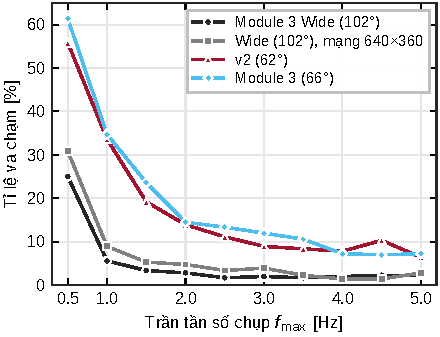
\includegraphics[width=0.5\textwidth]{Fig6.pdf}
\caption{Tỉ lệ va chạm với vật tĩnh theo trần tần số cho bốn cấu hình camera (SN, COV và FR gộp, 360 lượt mỗi điểm)}
\label{fig:cam}
\end{figure}

% =====================================================================================================
\section{Thảo luận}\label{sec:discussion}

\subsection{Ý nghĩa và vị trí so với các công trình trước}

Lợi ích của việc loại bỏ 28--50\,\% số lần suy luận nên được hiểu theo tài nguyên của bộ tăng tốc chứ không theo năng lượng bay: trên MAV được khảo sát ở~\cite{boroujerdian2021}, tính toán chiếm dưới 0.05\,\% tổng năng lượng. Phần tính toán được giải phóng có thể dành cho các tác vụ dùng chung CPU/GPU~\cite{wofk2019}, cho một mạng lớn hơn ở cùng tần số trung bình, hoặc làm dự trữ cho các đoạn dày. So với Zhuyi và D3~\cite{hsiao2022,gog2022}, điều kiện phủ không suy nhu cầu nhận thức từ các vật đã phát hiện mà từ phần không gian chưa quan sát dọc đường đi, nên xét trực tiếp vùng bị che mà~\cite{hsiao2022} để ngỏ; RoboRun đặt hạn chót quyết định từ tầm nhìn và quãng dừng và điều chỉnh tần số quyết định theo sự không đồng nhất của không gian~\cite{boroujerdian2021}, không dựa vào vùng chưa quan sát dọc đường đi. So với các bộ lập kế hoạch giữ quỹ đạo dừng trong vùng đã biết~\cite{liu2016,tordesillas2021}, nó dùng cùng lập luận để quyết định khi nào đo. So với RAPTOR~\cite{zhou2021}, vốn điều chỉnh quỹ đạo và góc yaw để điểm đường đi rời vùng đã biết là trống được quan sát đủ sớm để dừng, điều kiện phủ để chuyển động cho bộ lập kế hoạch và quyết định khi nào chạy suy luận. So với NanoMap~\cite{florence2018}, phép thử vùng trống giống nhau, nhưng ở đây nó quyết định thời điểm suy luận. Sự bão hoà của tỉ lệ va chạm từ khoảng 2~Hz phù hợp với các quan sát ở xe tự hành rằng tần số xử lý cần thiết là hữu hạn và phụ thuộc kịch bản~\cite{zhao2021,hsiao2022}.

\subsection{Phạm vi và hạn chế}

\begin{itemize}
\item \emph{Mô phỏng.} Mạng depth được thay bằng mô hình sai số tổng hợp trên ảnh depth dò tia (không dựng ảnh màu, không có mặt đất), và thông số camera lấy từ thông số công bố. Kết quả cần được kiểm chứng trên phần cứng, nơi nhiều công trình liên quan đã bay thật~\cite{loquercio2021,simon2023,tordesillas2021,pant2021}.
\item \emph{Bảo đảm.} Mệnh đề~\ref{prop:cov} là điều kiện cục bộ cho quyết định lập lịch, dưới giả thiết vùng trống quan sát đúng và tốc độ không tăng trong $\tauh$; \eqref{eq:need} không chứa số hạng gia tốc. Vòng kín không có chứng nhận hình thức (Nhận xét~\ref{rem:scope}): bộ lọc CBF rời rạc ở 100~Hz nên an toàn giữa các bước không được bảo đảm hình thức~\cite{breeden2022,bahati2024}; bộ lọc dùng biến bù~\cite{yaghoubi2021}; bán kính phồng nhảy tại mỗi lần cập nhật Kalman; và MPC với ràng buộc dừng cuối và hàng CBF ở vài bước đầu không có chứng minh khả thi đệ quy~\cite{zeng2021}.
\item \emph{Vật tĩnh.} Phương tiện cắt ngang trong SH chỉ được cập nhật vị trí theo từng khung; 56 va chạm với chúng ở trần từ 1.5~Hz nằm ngoài phạm vi.
\item \emph{Va chạm còn lại.} Từ 2~Hz, tỉ lệ va chạm gộp bốn bộ lập lịch là 2.4--3.2\,\% trên SN và 8.3\,\% trên SH và không giảm khi tăng trần (Mục~\ref{sec:r1}); mức nền này không do tần số nhận thức, và việc phân tích nguồn gốc của nó nằm ngoài phạm vi bài.
\item \emph{Cảnh dày liên tục.} Trên SH, COV có tỉ lệ va chạm 8.2\,\% so với 5.8\,\% của FR ($p = 0.098$); dữ liệu không cho phép khẳng định tương đương trong loại cảnh này.
\item \emph{Biểu diễn.} Hình trụ đứng bảo thủ với vật dài theo phương ngang nhìn chéo; phương thẳng đứng lấy từ tư thế thật tại thời điểm chụp; tầm $\Reff$ được đo trước khi chuyển sang mô hình hình trụ.
\end{itemize}

% =====================================================================================================
\section{Kết luận}\label{sec:conclusion}

Bài báo đặt câu hỏi khi nào một quadrotor chi phí thấp cần chạy mạng depth đơn mắt có độ trễ, và trả lời bằng một điều kiện hình học: khi đoạn đường đi dự kiến, tới quãng cần để dừng sau kết quả kế tiếp, không còn nằm trong vùng trống đã quan sát. Điều kiện này đủ để việc bỏ qua suy luận không làm mất khả năng dừng trong vùng đã quan sát. Kết hợp với trần tần số cứng và giới hạn tốc độ theo tầm cảm nhận, nó cho các hệ quả được kiểm chứng trên 36\,000 lượt mô phỏng: ở cùng trần, số suy luận giảm 28--50\,\% trên kịch bản thường và đời thường mà không có khác biệt an toàn có ý nghĩa; tần số chụp tăng theo mật độ vật cản; ở cùng số suy luận, tiêu chí hình học cho tỉ lệ va chạm thấp hơn tiêu chí thời gian an toàn còn lại; ở cùng ngân sách thấp, số lượt thất bại giảm. Điều kiện để các kết quả này đứng vững là camera góc nhìn rộng với mạng độ trễ thấp. Các bước tiếp theo là đưa số hạng gia tốc vào điều kiện phủ và kiểm chứng trên phần cứng.

% =====================================================================================================
\section*{Khai báo}

\paragraph{Tài trợ.} \todo{Ví dụ: Không có tài trợ cho nghiên cứu này.}
\paragraph{Xung đột lợi ích.} \todo{Ví dụ: Các tác giả không có xung đột lợi ích liên quan tới nội dung bài báo.}
\paragraph{Dữ liệu.} Kết quả từng lượt và các script lập bảng, vẽ hình có tại kho \url{https://github.com/nxbnxb1/project1} \todo{lưu bản phát hành cố định trên Zenodo để có DOI và trích dẫn DOI đó}.
\paragraph{Mã nguồn.} Mã MATLAB/Simulink và các workflow GitHub Actions có tại cùng kho.
\paragraph{Đóng góp của tác giả.} \todo{Theo CRediT.}
\paragraph{Sử dụng công cụ AI.} \todo{Tác giả hoàn thiện theo Mục 8 của docs/paper/PLAN.md.}

\begin{thebibliography}{99}
\small
% generated by docs/paper/build_refs.py - do not edit
\bibitem{falanga2019} Falanga, D., Kim, S., Scaramuzza, D.: How fast is too fast? The role of perception latency in high-speed sense and avoid. IEEE Robot. Autom. Lett. \textbf{4}(2), 1884--1891 (2019). \url{https://doi.org/10.1109/LRA.2019.2898117}

\bibitem{loquercio2021} Loquercio, A., Kaufmann, E., Ranftl, R., M\"uller, M., Koltun, V., Scaramuzza, D.: Learning high-speed flight in the wild. Sci. Robot. \textbf{6}(59), eabg5810 (2021). \url{https://doi.org/10.1126/scirobotics.abg5810}

\bibitem{yang2024b} Yang, L., Kang, B., Huang, Z., Zhao, Z., Xu, X., Feng, J., Zhao, H.: Depth Anything V2. In: Adv. Neural Inf. Process. Syst. (NeurIPS) \textbf{37}, 21875--21911 (2024). \url{https://doi.org/10.52202/079017-0688}

\bibitem{wofk2019} Wofk, D., Ma, F., Yang, T.-J., Karaman, S., Sze, V.: FastDepth: Fast monocular depth estimation on embedded systems. In: Proc. Int. Conf. Robot. Autom. (ICRA), pp. 6101--6108 (2019). \url{https://doi.org/10.1109/ICRA.2019.8794182}

\bibitem{simon2023} Simon, N., Majumdar, A.: MonoNav: MAV navigation via monocular depth estimation and reconstruction. In: Ang Jr, M.H., Khatib, O. (eds.) Experimental Robotics (ISER 2023). Springer Proc. Adv. Robot., pp. 415--426. Springer, Cham (2024). \url{https://doi.org/10.1007/978-3-031-63596-0_37}

\bibitem{liu2016} Liu, S., Watterson, M., Tang, S., Kumar, V.: High speed navigation for quadrotors with limited onboard sensing. In: Proc. IEEE Int. Conf. Robot. Autom. (ICRA), pp. 1484--1491 (2016). \url{https://doi.org/10.1109/ICRA.2016.7487284}

\bibitem{zhao2021} Zhao, H., Hari, S.K.S., Tsai, T., Sullivan, M.B., Keckler, S.W., Zhao, J.: Suraksha: A framework to analyze the safety implications of perception design choices in AVs. In: Proc. IEEE 32nd Int. Symp. Softw. Reliab. Eng. (ISSRE), pp. 434--445 (2021). \url{https://doi.org/10.1109/ISSRE52982.2021.00052}

\bibitem{hsiao2022} Hsiao, Y.-S., Hari, S.K.S., Filipiuk, M., Tsai, T., Sullivan, M.B., Reddi, V.J., Singh, V., Keckler, S.W.: Zhuyi: Perception processing rate estimation for safety in autonomous vehicles. In: Proc. 59th ACM/IEEE Design Autom. Conf. (DAC), pp. 289--294 (2022). \url{https://doi.org/10.1145/3489517.3530445}

\bibitem{gog2022} Gog, I., Kalra, S., Schafhalter, P., Gonzalez, J.E., Stoica, I.: D3: A dynamic deadline-driven approach for building autonomous vehicles. In: Proc. 17th Eur. Conf. Comput. Syst. (EuroSys), pp. 453--471 (2022). \url{https://doi.org/10.1145/3492321.3519576}

\bibitem{boroujerdian2021} Boroujerdian, B., Ghosal, R., Cruz, J., Plancher, B., Reddi, V.J.: RoboRun: A robot runtime to exploit spatial heterogeneity. In: Proc. 58th ACM/IEEE Design Autom. Conf. (DAC), pp. 829--834 (2021). \url{https://doi.org/10.1109/DAC18074.2021.9586280}

\bibitem{pant2021} Pant, Y.V., Abbas, H., Mohta, K., Quaye, R.A., Nghiem, T.X., Devietti, J., Mangharam, R.: Anytime computation and control for autonomous systems. IEEE Trans. Control Syst. Technol. \textbf{29}(2), 768--779 (2021). \url{https://doi.org/10.1109/TCST.2020.2979388}

\bibitem{tordesillas2021} Tordesillas, J., Lopez, B.T., Everett, M., How, J.P.: FASTER: Fast and safe trajectory planner for navigation in unknown environments. IEEE Trans. Robot. \textbf{38}(2), 922--938 (2022). \url{https://doi.org/10.1109/TRO.2021.3100142}

\bibitem{florence2018} Florence, P.R., Carter, J., Ware, J., Tedrake, R.: NanoMap: Fast, uncertainty-aware proximity queries with lazy search over local 3D data. In: Proc. IEEE Int. Conf. Robot. Autom. (ICRA), pp. 7631--7638 (2018). \url{https://doi.org/10.1109/ICRA.2018.8463195}

\bibitem{aldana2023} Aldana-L\'opez, R., Arag\"u\'es, R., Sag\"u\'es, C.: Latency vs precision: Stability preserving perception scheduling. Automatica \textbf{155}, 111123 (2023). \url{https://doi.org/10.1016/j.automatica.2023.111123}

\bibitem{huang2020} Huang, C., Xu, S., Wang, Z., Lan, S., Li, W., Zhu, Q.: Opportunistic intermittent control with safety guarantees for autonomous systems. In: Proc. 57th ACM/IEEE Design Autom. Conf. (DAC), pp. 1--6 (2020). \url{https://doi.org/10.1109/DAC18072.2020.9218742}

\bibitem{zhou2019} Zhou, B., Gao, F., Wang, L., Liu, C., Shen, S.: Robust and efficient quadrotor trajectory generation for fast autonomous flight. IEEE Robot. Autom. Lett. \textbf{4}(4), 3529--3536 (2019). \url{https://doi.org/10.1109/LRA.2019.2927938}

\bibitem{lin2020} Lin, J., Zhu, H., Alonso-Mora, J.: Robust vision-based obstacle avoidance for micro aerial vehicles in dynamic environments. In: Proc. IEEE Int. Conf. Robot. Autom. (ICRA), pp. 2682--2688 (2020). \url{https://doi.org/10.1109/ICRA40945.2020.9197481}

\bibitem{falanga2018} Falanga, D., Foehn, P., Lu, P., Scaramuzza, D.: PAMPC: Perception-aware model predictive control for quadrotors. In: Proc. IEEE/RSJ Int. Conf. Intell. Robots Syst. (IROS), pp. 1--8 (2018). \url{https://doi.org/10.1109/IROS.2018.8593739}

\bibitem{misyats2025} Misyats, M., Harms, M., Nissov, M., Jacquet, M., Alexis, K.: Embedded safe reactive navigation for multirotors systems using control barrier functions. In: Proc. Int. Conf. Unmanned Aircr. Syst. (ICUAS), pp. 697--704 (2025). \url{https://doi.org/10.1109/ICUAS65942.2025.11007827}

\bibitem{ames2017} Ames, A.D., Xu, X., Grizzle, J.W., Tabuada, P.: Control barrier function based quadratic programs for safety critical systems. IEEE Trans. Autom. Control \textbf{62}(8), 3861--3876 (2017). \url{https://doi.org/10.1109/TAC.2016.2638961}

\bibitem{ames2019} Ames, A.D., Coogan, S., Egerstedt, M., Notomista, G., Sreenath, K., Tabuada, P.: Control barrier functions: Theory and applications. In: Proc. 18th Eur. Control Conf. (ECC), pp. 3420--3431 (2019). \url{https://doi.org/10.23919/ECC.2019.8796030}

\bibitem{wang2017} Wang, L., Ames, A.D., Egerstedt, M.: Safety barrier certificates for collisions-free multirobot systems. IEEE Trans. Robot. \textbf{33}(3), 661--674 (2017). \url{https://doi.org/10.1109/TRO.2017.2659727}

\bibitem{xiao2019} Xiao, W., Belta, C.: Control barrier functions for systems with high relative degree. In: Proc. IEEE 58th Conf. Decis. Control (CDC), pp. 474--479 (2019). \url{https://doi.org/10.1109/CDC40024.2019.9029455}

\bibitem{zeng2021} Zeng, J., Zhang, B., Sreenath, K.: Safety-critical model predictive control with discrete-time control barrier function. In: Proc. Am. Control Conf. (ACC), pp. 3882--3889 (2021). \url{https://doi.org/10.23919/ACC50511.2021.9483029}

\bibitem{rosolia2020} Rosolia, U., Ames, A.D.: Multi-rate control design leveraging control barrier functions and model predictive control policies. IEEE Control Syst. Lett. \textbf{5}(3), 1007--1012 (2021). \url{https://doi.org/10.1109/LCSYS.2020.3008326}

\bibitem{breeden2022} Breeden, J., Garg, K., Panagou, D.: Control barrier functions in sampled-data systems. IEEE Control Syst. Lett. \textbf{6}, 367--372 (2022). \url{https://doi.org/10.1109/LCSYS.2021.3076127}

\bibitem{bahati2024} Bahati, G., Ong, P., Ames, A.D.: Sample-and-hold safety with control barrier functions. In: Proc. Am. Control Conf. (ACC), pp. 5169--5176 (2024). \url{https://doi.org/10.23919/ACC60939.2024.10645060}

\bibitem{molnar2022} Molnar, T.G., Kiss, A.K., Ames, A.D., Orosz, G.: Safety-critical control with input delay in dynamic environment. IEEE Trans. Control Syst. Technol. \textbf{31}(4), 1507--1520 (2023). \url{https://doi.org/10.1109/TCST.2022.3227451}

\bibitem{taylor2020} Taylor, A.J., Ong, P., Cort\'es, J., Ames, A.D.: Safety-critical event triggered control via input-to-state safe barrier functions. IEEE Control Syst. Lett. \textbf{5}(3), 749--754 (2021). \url{https://doi.org/10.1109/LCSYS.2020.3005101}

\bibitem{yang2019} Yang, G., Belta, C., Tron, R.: Self-triggered control for safety critical systems using control barrier functions. In: Proc. Am. Control Conf. (ACC), pp. 4454--4459 (2019). \url{https://doi.org/10.23919/ACC.2019.8814657}

\bibitem{dean2021} Dean, S., Taylor, A.J., Cosner, R.K., Recht, B., Ames, A.D.: Guaranteeing safety of learned perception modules via measurement-robust control barrier functions. In: Proc. 2020 Conf. Robot Learning (CoRL), PMLR \textbf{155}, 654--670 (2021)

\bibitem{yang2023} Yang, S., Pappas, G.J., Mangharam, R., Lindemann, L.: Safe perception-based control under stochastic sensor uncertainty using conformal prediction. In: Proc. 62nd IEEE Conf. Decis. Control (CDC), pp. 6072--6078 (2023). \url{https://doi.org/10.1109/CDC49753.2023.10384075}

\bibitem{yaghoubi2021} Yaghoubi, S., Fainekos, G., Yamaguchi, T., Prokhorov, D., Hoxha, B.: Risk-bounded control with Kalman filtering and stochastic barrier functions. In: Proc. 60th IEEE Conf. Decis. Control (CDC), pp. 5213--5219 (2021). \url{https://doi.org/10.1109/CDC45484.2021.9683756}

\bibitem{zhu2019} Zhu, H., Alonso-Mora, J.: Chance-constrained collision avoidance for MAVs in dynamic environments. IEEE Robot. Autom. Lett. \textbf{4}(2), 776--783 (2019). \url{https://doi.org/10.1109/LRA.2019.2893494}

\bibitem{laine2020} Laine, F., Chiu, C.-Y., Tomlin, C.: Eyes-closed safety kernels: Safety of autonomous systems under loss of observability. In: Robotics: Science and Systems XVI (2020). \url{https://doi.org/10.15607/RSS.2020.XVI.096}

\bibitem{barshalom2002} Bar-Shalom, Y.: Update with out-of-sequence measurements in tracking: Exact solution. IEEE Trans. Aerosp. Electron. Syst. \textbf{38}(3), 769--777 (2002). \url{https://doi.org/10.1109/TAES.2002.1039398}

\bibitem{garcia2021} Garc\'ia-Fern\'andez, \'A.F., Yi, W.: Continuous-discrete multiple target tracking with out-of-sequence measurements. IEEE Trans. Signal Process. \textbf{69}, 4699--4709 (2021). \url{https://doi.org/10.1109/TSP.2021.3100999}

\bibitem{rpi_cm3} Raspberry Pi Ltd: Raspberry Pi Camera Module 3 (Standard, NoIR, Wide, NoIR Wide), product brief (2024). \url{https://datasheets.raspberrypi.com/camera/camera-module-3-product-brief.pdf}

\bibitem{ranftl2020} Ranftl, R., Lasinger, K., Hafner, D., Schindler, K., Koltun, V.: Towards robust monocular depth estimation: Mixing datasets for zero-shot cross-dataset transfer. IEEE Trans. Pattern Anal. Mach. Intell. \textbf{44}(3), 1623--1637 (2022). \url{https://doi.org/10.1109/TPAMI.2020.3019967}

\bibitem{yang2024a} Yang, L., Kang, B., Huang, Z., Xu, X., Feng, J., Zhao, H.: Depth Anything: Unleashing the power of large-scale unlabeled data. In: Proc. IEEE/CVF Conf. Comput. Vis. Pattern Recognit. (CVPR), pp. 10371--10381 (2024). \url{https://doi.org/10.1109/CVPR52733.2024.00987}

\bibitem{bhattacharya2024} Bhattacharya, A., Cannici, M., Rao, N., Tao, Y., Kumar, V., Matni, N., Scaramuzza, D.: Monocular event-based vision for obstacle avoidance with a quadrotor. In: Proc. 8th Conf. Robot Learning (CoRL), PMLR \textbf{270}, 4826--4843 (2025)

\bibitem{mehrotra1992} Mehrotra, S.: On the implementation of a primal--dual interior point method. SIAM J. Optim. \textbf{2}(4), 575--601 (1992). \url{https://doi.org/10.1137/0802028}


\end{thebibliography}

\end{document}
